% Document uses 12 pt font
% 1 in margins
% Contains a relative path for images

\documentclass [10pt]{article}

% page geometry 
\usepackage[margin=1in]{geometry}


% ----------  PACKAGES START ------------ %
% Math Packages
\usepackage{amsmath}
\usepackage{mathtools}

% Table cell color package and highlighting
\usepackage[table,xcdraw]{xcolor}
\usepackage{color,soul}


% VIC title package
%\usepackage{cabin}
\usepackage[T1]{fontenc}

% default font package
%\usepackage{times}
\usepackage{helvet}
%\renewcommand{\familydefault}{\sfdefault}

% ---------- End Font Packages -------------- %

\usepackage{listings}
\usepackage{float}

%\definecolor{dkgreen}{rgb}{0,0.6,0}
%\definecolor{gray}{rgb}{0.5,0.5,0.5}
%\definecolor{mauve}{rgb}{0.58,0,0.82}

\lstset{frame=tb,
  language=C++,
  aboveskip=3mm,
  belowskip=3mm,
  showstringspaces=false,
  columns=flexible,
  basicstyle={\small\ttfamily},
  numbers=none,
  numberstyle=\tiny\color{gray},
  keywordstyle=\color{blue},
  commentstyle=\color{dkgreen},
  stringstyle=\color{mauve},
  breaklines=true,
  breakatwhitespace=true,
  tabsize=3
}

% Title Packages
\usepackage{titlesec}
\usepackage{titletoc}

% Image Package
\usepackage{graphicx}

% Table Packages
\usepackage{longtable}
\usepackage{multirow}
\usepackage{multicol}
\usepackage{multirow}
\usepackage{array}
\renewcommand{\arraystretch}{1.2}% Spread rows out evenly in table
\setlength{\LTpre}{0.5pt} % Reduces white space around tables (top)
%\setlength{\LTpost}{0pt} % Reduces white space around tables (bottom)

% Color Packages
\usepackage{color}   
\definecolor{sectionC}{rgb}{0.95,0.52,.0}
\definecolor{subsectionC}{rgb}{1.0,.64,.26}
\definecolor{subsubsectionC}{rgb}{1.0,.87,.68}
\definecolor{tableCell}{rgb}{.98,.81,.69}


% List package
\usepackage{enumitem}
\setenumerate{itemsep=0pt, itemindent=0in,leftmargin=0.5in}


% Paragraph parameter

\setlength{\parindent}{0pt}


% ------------- Creates a linked Table of Contents  Start --------------- %
\usepackage{hyperref}
\hypersetup{
colorlinks=true, %set true if you want colored links
linktoc=all,     %set to all if you want both sections and subsections linked
linkcolor=black,}  %choose some color if you want links to stand out

% ------------- Creates a click-able Table of Contents  End--------------- %

% ---------- PACKAGES END ------------ %








% -------- SECTION AND SUBSECTION FORMATING START -------- % 
% starts the 
%\setcounter{section}{1}


\titleformat{\section} % Section
{\normalfont \fontsize{14}{14} \bfseries}{}{0em}{\colorsection}

% Makes a background color
\newcommand{\colorsection}[1]{%
  \colorbox{sectionC}{\parbox{\dimexpr\textwidth-1\fboxsep}{\color{white}\Large\thesection\ \hspace{1mm} #1}}}

% Makes a background color
\titleformat{\subsection} % Subsection
{\normalfont \fontsize{12}{12}  \bfseries}{}{0em}{\colorsubsection }

\newcommand{\colorsubsection}[1]{%
  \colorbox{subsectionC}{\parbox{\dimexpr \textwidth -1\fboxsep}{\large\thesubsection\ #1}}}


% Makes a background color
\titleformat{\subsubsection} % Subsubsection
{\normalfont \fontsize{12}{12} \bfseries}{}{0em}{\colorsubsubsection}

\newcommand{\colorsubsubsection}[1]{%
  \colorbox{subsubsectionC}{\parbox{\dimexpr\textwidth-1\fboxsep}{\thesubsubsection\ #1}}}

% -------- SECTION AND SUBSECTION FORMATING END -------- % 
\usepackage{lipsum}


% -----  IMAGE PATH START -----%
% Relative Image Path
\graphicspath {figures/}
% -----  IMAGE PATH END -----%

% ------ PARAGRAPH FORMAT START ----%
%\setlength{\parskip}{.2em}% Sets the space between new paragraph items 
\setlength{\parindent}{0em} % paragraph indent
% ------ PARAGRAPH FORMAT END ----%




%------------------------------TOC FORMAT START --------------------------------%
\usepackage{tocloft}



% Section indentations
\cftsetindents{section}{0em}{1.5em}
\cftsetindents{subsection}{1em}{2em}
\cftsetindents{subsubsection}{2em}{3em}

% Toc title size
\renewcommand\cfttoctitlefont{\Large\bfseries}
\renewcommand*\contentsname{Table of Contents}

\newcommand{\carSpeed}{1.4\ m/s}
\newcommand{\intersectionLength}{0.6\ m}


% Removes bold headings from toc
%\renewcommand{\cftsecfont}{\normalfont}

% Removes bold heading page numbers from toc
\renewcommand{\cftsecpagefont}{\normalfont}

% add dots after headings
%\renewcommand{\cftsecleader}{\cftdotfill{\cftdotsep}} 


% number of section headings we want to see in toc
\setcounter{tocdepth}{2}

% Spaceing before headings in toc
\setlength{\cftbeforesecskip}{6pt}

% ------------------------------TOC FORMAT END --------------------------------%



% ------------------- START HEADER AND FOOTER ---------------------------%
\usepackage{fancyhdr}

% Helps with the n of total n pages
\usepackage{lastpage}

\pagestyle{fancy}

% Header
\lhead{Design Document}
\rhead{Revision: 2}
\fancyhead[LE,CO]{Group 9: LazyBots}

% Removes line under the header 
\renewcommand{\headrulewidth}{0pt}
\setlength{\headsep}{.2in}

% Footer 

% Set the right side of the footer to be the page number
\fancyfoot[R]{Page \textbf{\thepage}\ of \textbf{\pageref{LastPage}}}
\fancyfoot[C]{}

% ------------------- END HEADER AND FOOTER ---------------------------%






% -------------- DOCUMENT START ---------------%
\begin{document}

% --------- TITLE PAGE START ------- %
\begin {center} 

\thispagestyle{empty}
\vspace*{5cm}

% Logo Insertion
\begin {figure}[h!]
\centering
\hspace{-10mm}
\includegraphics [scale = .3, trim={.4cm 0 .8cm 0},clip] {figures/alfred.png}
\end {figure}

{%\fontfamily{\cabinfamily}\selectfont
\Huge{LazyBots} }

\vspace{1 cm}
{\Large\textbf{\textsc{McMaster University}}\\}  \vspace {1cm}
{\Large Design Document \\ \vspace {0.4 cm} SE 4GA6 \& TRON 4TB6}  \vspace {1cm}

{\large \textsc{Group 9} \\} \vspace{1cm}



\begin{tabular}{ l c  l}
Karim Guirguis & & 001307668 \\
David Hemms & & 001309228 \\
Marko Laban & & 001300989 \\
Curtis Milo & & 001305877 \\
Keyur Patel & & 001311559 \\
Alexandra Rahman & & 001305735
\end{tabular}


\end{center}


% --------- TITLE PAGE END------- %

\pagebreak

% Inserting table of contents and table of figures 

\tableofcontents
\listoftables
\listoffigures



\pagebreak

% -----------  REVISION HISTORY START ----------- %

%\section*{Revisions}
\thispagestyle{empty}
\section{Revisions}
\begin{longtable}{| p{.2\textwidth } | p{.23\textwidth } | p{.23\textwidth } | p{.23\textwidth } |}

\hline 
\centering \textbf{Date} & 
\multicolumn{1}{c}{\textbf {Revision Number}} &
\multicolumn{1}{|c}{\textbf {Authors}} & 
\multicolumn{1}{|c|}{\textbf {Comments}} \\ \hline

\multirow{5}{*}{\centering December 24\textsuperscript{th}, 2017}  & 
\multirow{5}{*}{Revision 0}& 
		{Karim Guirguis \newline
		David Hemms \newline
		Marko Laban \newline
		Curtis Milo \newline
		Keyur Patel \newline
		Alexandra Rahman} &
 
\multirow{4}{*}{-} \\ 
\hline 


\multirow{7}{*}{\centering March 12\textsuperscript{th}, 2018}  & 
\multirow{7}{*}{Revision 1}& 
		{Karim Guirguis \newline
		David Hemms \newline
		Marko Laban \newline
		Curtis Milo \newline
		Keyur Patel \newline
		Alexandra Rahman} &
{Added the section to include the assumptions of the project as well as added some traceability between the components and the requirements. Finally, included the components that were likely to change. }\\
\hline

\multirow{5}{*}{\centering March 16\textsuperscript{th}, 2018}  & 
\multirow{5}{*}{Revision 2}& 
		{Karim Guirguis \newline
		David Hemms \newline
		Marko Laban \newline
		Curtis Milo \newline
		Keyur Patel \newline
		Alexandra Rahman} &
{Combined System Design Document and Component Design Document and updated the MIS, MID and Design Notes.}\\
\hline 

\caption{LazyBots Table of Revisions} 
\end{longtable}



\pagebreak

%---------------------------- PROJECT DRIVERS ------------------------%
% heading in document

% -------------- START INTRODUCTION ---------------- %

% ------------------------------------------------------- PURPOSE ------------------------------------------------------- %
\section {Purpose}

The purpose of this project will be to create an autonomous robot that will navigate to and serve
the requested drink to the user who request a drink. Currently in an office setting, workers must
leave their offices to get their own drinks. In restaurants, drinks are served by waiters and
waitresses, which hinders them from doing other work at that time. Alfred will be designed to make the serving drinks autonomous.\newline

Alfred will allow users to request drinks. These requests will form a queue which Alfred will serve in order using a FIFO protocol. Alfred will go to the table of each user and pour the drinks ordered from that table. Alfred will also have an administrator user which will be able to call Alfred back and override any action that is being taken at the time.\newline

The following document will outline the overall system components, as well as the overall system behaviour, operation and undesired error handling.

% ------------------------------------------------------- Scope ------------------------------------------------------- %

\subsection{Scope}

The system implemented is one that is meant to automate the dispensing of beverages to customers within a restaurant at the respective customers' table. The customer will be able to order a drink from their table which will be relayed to Alfred, where he will arrive at their table and dispense the requested drinks. The staff will be able to request Alfred to come back for charging and refilling when desired.


% ------------------------------------------------------- Context Diagram ------------------------------------------------------- %

\subsection{Context Diagram}
Figure 1 is a context diagram of the drink serving robot, Alfred.
\begin{figure} [h!]
	\centering
	\includegraphics [scale = 0.5] {Figures/ContextDiagram.png}
	\caption{Drink Serving Robot Context Diagram}
\end{figure}

% ---------------------------------------------------- Diagram of Components ----------------------------------------------------- %

\subsection{Diagram of Components}
Figure 2 is a diagram that shows the interaction of components of the drink serving robot system.
\begin{figure} [h!]
	\centering
	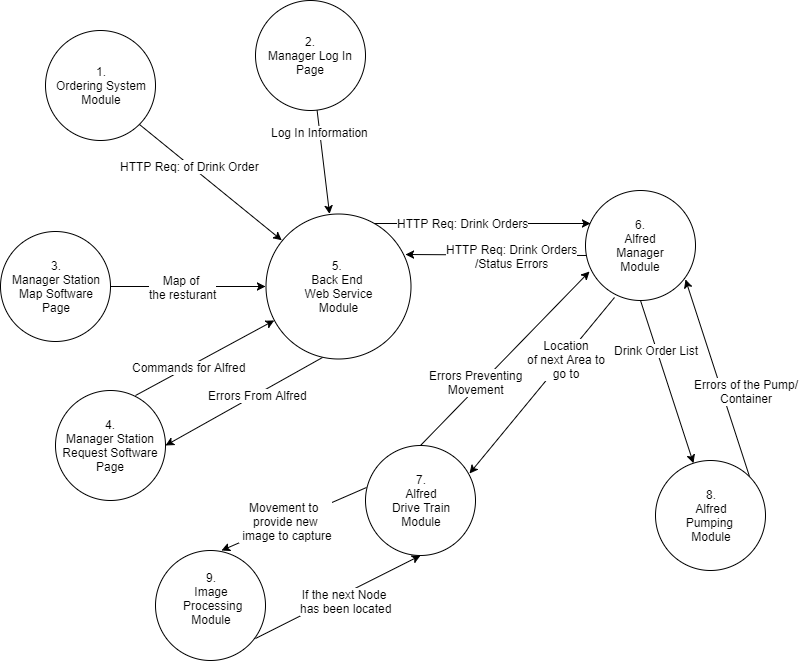
\includegraphics [scale = 0.6] {Figures/SystemComponents.png}
	\caption{Drink Serving Robot System Component Diagram}
\end{figure}

% ------------------------------------------------------------ Assumptions ------------------------------------------------------------- %

\subsection{Assumptions}

Alfred's assumption are represented in the tables below.  \\

% ------------------------------ Assumption 1 ------------------------------ %
\begin{longtable}{| p{.15\textwidth } | p{.80\textwidth } | }\hline 
\rowcolor{tableCell}\textbf{A1} & The environment will only be comprised of a one story building with no steps. \\ \hline
\textbf{Rationale} & Different environment elevations are beyond the scope of the project. Alfred will not be able to navigate around steps.\\ \hline 
\end{longtable}

\pagebreak 

% ------------------------------ Assumption 2 ------------------------------ %
\begin{longtable}{| p{.15\textwidth } | p{.80\textwidth } | }\hline 
\rowcolor{tableCell}\textbf{A2} & The ground within the establishment will be smooth without defect and with moderate friction. \\ \hline
\textbf{Rationale} & Imperfect floors with too much or too little friction are beyond the scope of the project. Alfred will not be able to navigate properly with imperfect floors and the wheels will slip with too little friction. \\ \hline 
\end{longtable}

% ------------------------------ Assumption 3 ------------------------------ %
\begin{longtable}{| p{.15\textwidth } | p{.80\textwidth } | }\hline 
\rowcolor{tableCell}\textbf{A3} & The establishment will be well light with a drop ceiling of a maximum height of 9 feet.  \\ \hline
\textbf{Rationale} & Poor lighting and different ceiling heights are beyond the scope of the project. A level ceiling is needed for node placement as  well as proper lighting will be needed so that Alfred will be able to read the nodes. \\ \hline 
\end{longtable}

% ------------------------------ Assumption 4 ------------------------------ %
\begin{longtable}{| p{.15\textwidth } | p{.80\textwidth } | }\hline 
\rowcolor{tableCell}\textbf{A4} & The establishment will be able to support a strong and stable Wi-Fi connection (internet connection).  \\ \hline
\textbf{Rationale} & Poor internet connections are beyond the scope of the project. To support communication between all components a strong and stable internet connection is needed.\\ \hline 
\end{longtable}

% ------------------------------ Assumption 5 ------------------------------ %
\begin{longtable}{| p{.15\textwidth } | p{.80\textwidth } | }\hline 
\rowcolor{tableCell}\textbf{A5} & The width of the walkways will be wide enough to accommodate all people. \\ \hline
\textbf{Rationale} &  If a table is not accessible to a human, it will not be accessible for Alfred.\\ \hline
\end{longtable}

% ------------------------------ Assumption 6 ------------------------------ %
\begin{longtable}{| p{.15\textwidth } | p{.80\textwidth } | }\hline 
\rowcolor{tableCell}\textbf{A6} & Orders will be placed via an Android or iOS application. \\ \hline
\textbf{Rationale} &  Eliminates the need for human interactions, making Alfred completely autonomous. \\ \hline
\end{longtable}

% ------------------------------ Assumption 7 ------------------------------ %
\begin{longtable}{| p{.15\textwidth } | p{.80\textwidth } | }\hline 
\rowcolor{tableCell}\textbf{A7} & The height of a table will not exceed 30". \\ \hline
\textbf{Rationale} &  This will help simplify the scope of the project and reduce the customers' discomfort when reaching for a drink.\\ \hline
\end{longtable}

% ------------------------------ Assumption 8 ------------------------------ %
\begin{longtable}{| p{.15\textwidth } | p{.80\textwidth } | }\hline 
\rowcolor{tableCell}\textbf{A8} & The serving size of a medium sized cup will not vary largely in terms of ounces. \\ \hline
\textbf{Rationale} &  The standard ounces in a cup will be restricted to 12oz. to accommodate as many users as possible and to limit the scope. \\ \hline
\end{longtable}


\subsection{Components to Requirements}



% ------------------------------------------------------- SYSTEM VARIABLES ------------------------------------------------------- %

\section{System Variables}

% ---------------------------------------------- Monitored and Controlled Variables ----------------------------------------------- %

\subsection{Monitored and Controlled Variables}
The following is a list of variables that will be monitored. \\

\begin{longtable}{|l|l|l|l|l|}\hline 
	\rowcolor{tableCell}\textbf{Monitor Name} & \textbf{Monitor Type} & \textbf{Range} & \textbf{Units} & \textbf{Comment(s)} \\ \hline
	$ w_{wheel_{left}} $ & Speed & [0, $ 100 $]& rad/s &  Left Wheel Speed\\ \hline
	\rowcolor{tableCell}$ w_{wheel_{right}} $ & Speed & [0, $ 100 $]& rad/s & Right Wheel Speed \\ \hline
	$ m_{container} $ & Mass & [0, 1.0]& Kg &  Weight of the storage device  \\ \hline
	\rowcolor{tableCell}$ m_{drink} $    & Mass & [0, 1.0] & Kg &  Weight of the drink  \\ \hline
	$ b_{cuptaken } $ & Boolean & [0,1] & N/A & If the cup has been taken \\ \hline
	\rowcolor{tableCell}$  d_{objects} $ & Distance[] & [0, 10.0]& m & Set of distances to closest obstacle \\ \hline
	$  V_{batt} $ & Voltage & [0, 20.0]& m &  Voltage levels of batteries \\ \hline
\end{longtable}


The following is a list of variables that will be controlled. \\

\begin{longtable}{|l|l|l|l|l|}\hline 
	\rowcolor{tableCell}\textbf{Controlled Name} & \textbf{Controlled Type} & \textbf{Range} & \textbf{Units} & \textbf{Comment(s)} \\ \hline
    $w_{motor}$ & Speed & [0, $ 100 $]& rad/s &  Motor Speed\\ \hline
    	\rowcolor{tableCell}$ percent_{dutycycle_{left}} $ & Percent & [0,1.0] & \% & The duty cycle of the left side of the drive-train \\ \hline
    $ percent_{dutycycle_{right}} $ & Percent & [0, 1.0]& \% & The duty cycle of the right side of the drive-train\\ \hline
   \rowcolor{tableCell} $  V_{pump} $ & Voltage & [0, 5.0]& m &  Voltage going to the liquid pump \\ \hline
	$ errors_{drivetrain} $ & Unsigned Byte & [0, $2^{8}$]& N/A & Errors from drive-train \\ \hline
	\rowcolor{tableCell}$  errors_{pump} $ & Unsigned Byte & [0, $2^{8}$]& N/A & Errors from pumping system module \\ \hline
	$  errors_{Alfred} $ & Unsigned Byte & [0, $2^{8}$]& N/A & Errors from Alfred \\ \hline
	\rowcolor{tableCell}$LED_{drinksignal}$ & Boolean & [0, 1]& N/A & Signal of drink that it is ready to be picked up \\ \hline
	$Q_{pump}$ & Flow Rate & [0, $ 100 $]& ($m^3/s$) &  Flow rate of the pump\\ \hline
\end{longtable}


% ------------------------------------------------------- Constants ------------------------------------------------------- %

\subsection{Constants}

The following is a list of system constants. \\

\begin{longtable}{| p{0.2\textwidth} | p{0.15\textwidth} | p{0.05\textwidth} | p{0.08\textwidth} | p{.45\textwidth} |}\hline 
	\rowcolor{tableCell}\textbf{Constant Name} & \textbf{Constant Type} & \textbf{Value} & \textbf{Units} & \textbf{Comment(s)} \\ \hline
 	$ V_{battMin} $ & Voltage & 9.0& m &  The minimum voltage necessary for drive-train movement \\ \hline
	\rowcolor{tableCell}$ m_{DrinkMin} $ & Mass & 0.35 & Kg &  The minimum weight of the drink to be considered as ready for the customer.  \\ \hline
	$ t_{timeout} $ & Time & 30 & s & The maximum time Alfred or the ordering application will wait for a message from the server before timing out.  \\ \hline
	\rowcolor{tableCell}$ t_{pumptimeout} $ & Time & 5 & s & The maximum time Alfred will try to pump without noticing a change in the weight of the tank.  \\ \hline
	$ t_{maxpump} $ & Time & 10 & s & The maximum time Alfred will try to dispense a drink within. \\ \hline
	\rowcolor{tableCell}$Q_{pump}$ & Flow Rate & TBD & ($m^3/s$) &  Flow rate of the pump\\ \hline
	$ freq_{bauderate} $ & Frequency & 9600 & (Herts) &  The  rate at which UART communication will be performed at.\\ \hline
	\rowcolor{tableCell}$ obstruction_{timeout} $ & Time & 10 & s & The amount of time that Alfred will stop movement due to an object in its path before ruling that there is an obstruction and throwing an error. \\ \hline
\end{longtable}


% ----------------------------------------------------- BEHAVIOUR OVERVIEW ---------------------------------------------------- %

\section{Behaviour Overview}
\begin{enumerate}
	\item \textbf{Ordering System Module}: Provided the order information, this module will communicate with the server to "order a drink".
	\item \textbf{Manager Login Page}: Given the login credentials, will authenticate administrator of the system with the server.
	\item \textbf{Manager Station Map Software Page}: Will allow administrator to create or modify the map of the area where Alfred will deliver drinks. This map will then be sent and stored on the server.
	\item \textbf{Manager Station Request Software Page}: Will allow administrator to execute commands for Alfred, as well as view incoming error codes from Alfred. Said commands, will be sent to the server, which will then communicate with Alfred.
	\item \textbf{Back End Web Service Module}: Will route communication to different components of the system. Will also be responsible for authentication and management of queue. 
	\item \textbf{Alfred Manager Module}: Endpoint for communication with Alfred. Will manage communication with server, as well as send any errors that Alfred is experiencing.
	\item \textbf{Alfred Drive Train Module}: Responsible for driving and managing the motors based on desired route. Will also be sending errors preventing movement to Alfred Manager Module.
	\item \textbf{Alfred Pumping Module}: Will control pumping system in regards of when to pour, how long, rate of dispensing, etc. Will also be sending errors pertaining to the pump or container to Alfred Manager Module.
	\item \textbf{Image Processing Module}: Will detect any obstacles in the way as well as locate incoming nodes. Will communicate with Alfred Drive Train Module, to determine wether any required action based on results.
\end{enumerate}

% ------------------------------------------------ COMPONENT TRACEABILITY ------------------------------------------------- %

\section{Component Traceability}


\begin{table}[h!]
\centering
\begin{tabular}{lllll}
\cline{1-2}
\multicolumn{1}{|c|}{\textbf{Component Module:}} & \multicolumn{1}{c|}{\textbf{Functional and Non-Functional Requirement:}} &  &  &  \\ \cline{1-2}
\multicolumn{1}{|c|}{\multirow{9}{*}{Ordering System Module}} & \multicolumn{1}{l|}{Table Ordering Functional Requirement 1} &  &  &  \\ \cline{2-2}
\multicolumn{1}{|c|}{} & \multicolumn{1}{l|}{Table Ordering Functional Requirement 2} &  &  &  \\ \cline{2-2}
\multicolumn{1}{|c|}{} & \multicolumn{1}{l|}{Non Functional Requirement 4} &  &  &  \\ \cline{2-2}
\multicolumn{1}{|c|}{} & \multicolumn{1}{l|}{Non Functional Requirement 5} &  &  &  \\ \cline{2-2}
\multicolumn{1}{|c|}{} & \multicolumn{1}{l|}{Non Functional Requirement 8} &  &  &  \\ \cline{2-2}
\multicolumn{1}{|c|}{} & \multicolumn{1}{l|}{Non Functional Requirement 9} &  &  &  \\ \cline{2-2}
\multicolumn{1}{|c|}{} & \multicolumn{1}{l|}{Non Functional Requirement 15} &  &  &  \\ \cline{2-2}
\multicolumn{1}{|c|}{} & \multicolumn{1}{l|}{Non Functional Requirement 30} &  &  &  \\ \cline{2-2}
\multicolumn{1}{|c|}{} & \multicolumn{1}{l|}{Non Functional Requirement 32} &  &  &  \\ \cline{1-2}
\end{tabular}
\caption{Ordering System Traceability}
\end{table}



\begin{table}[h!]
\centering
\begin{tabular}{lllll}
\cline{1-2}
\multicolumn{1}{|c|}{\textbf{Component Module:}} & \multicolumn{1}{c|}{\textbf{Functional and Non-Functional Requirement:}} &  &  &  \\ \cline{1-2}
\multicolumn{1}{|l|}{\multirow{5}{*}{Manager Login Page Module}} & \multicolumn{1}{l|}{Non Functional Requirement 4} &  &  &  \\ \cline{2-2}
\multicolumn{1}{|l|}{} & \multicolumn{1}{l|}{Non Functional Requirement 5} &  &  &  \\ \cline{2-2}
\multicolumn{1}{|l|}{} & \multicolumn{1}{l|}{Non Functional Requirement 8} &  &  &  \\ \cline{2-2}
\multicolumn{1}{|l|}{} & \multicolumn{1}{l|}{Non Functional Requirement 9} &  &  &  \\ \cline{2-2}
\multicolumn{1}{|l|}{} & \multicolumn{1}{l|}{Non Functional Requirement 30} &  &  &  \\ \cline{1-2}
\end{tabular}
\caption{Manager Login Page Traceability}
\end{table}


\pagebreak


\begin{table}[h!]
\centering
\begin{tabular}{lllll}
\cline{1-2}
\multicolumn{1}{|c|}{\textbf{Component Module:}} & \multicolumn{1}{c|}{\textbf{Functional and Non-Functional Requirement:}} &  &  &  \\ \cline{1-2}
\multicolumn{1}{|l|}{\multirow{9}{*}{Manager Station Map Software Module}} & \multicolumn{1}{l|}{Administrator Functional Requirement 1} &  &  &  \\ \cline{2-2}
\multicolumn{1}{|l|}{} & \multicolumn{1}{l|}{Administrator Functional Requirement 2} &  &  &  \\ \cline{2-2}
\multicolumn{1}{|l|}{} & \multicolumn{1}{l|}{Non Functional Requirement 4} &  &  &  \\ \cline{2-2}
\multicolumn{1}{|l|}{} & \multicolumn{1}{l|}{Non Functional Requirement 5} &  &  &  \\ \cline{2-2}
\multicolumn{1}{|l|}{} & \multicolumn{1}{l|}{Non Functional Requirement 8} &  &  &  \\ \cline{2-2}
\multicolumn{1}{|l|}{} & \multicolumn{1}{l|}{Non Functional Requirement 9} &  &  &  \\ \cline{2-2}
\multicolumn{1}{|l|}{} & \multicolumn{1}{l|}{Non Functional Requirement 29} &  &  &  \\ \cline{2-2}
\multicolumn{1}{|l|}{} & \multicolumn{1}{l|}{Non Functional Requirement 30} &  &  &  \\ \cline{2-2}
\multicolumn{1}{|l|}{} & \multicolumn{1}{l|}{Non Functional Requirement 33} &  &  &  \\ \cline{1-2}
\end{tabular}
\caption{Manager Station Map Traceability}
\end{table}


\begin{table}[h!]
\centering
\begin{tabular}{lllll}
\cline{1-2}
\multicolumn{1}{|c|}{\textbf{Component Module:}} & \multicolumn{1}{c|}{\textbf{Functional and Non-Functional Requirement:}} &  &  &  \\ \cline{1-2}
\multicolumn{1}{|l|}{\multirow{11}{*}{Manager Station Request Software Module}} & \multicolumn{1}{l|}{Administrator Functional Requirement 3} &  &  &  \\ \cline{2-2}
\multicolumn{1}{|l|}{} & \multicolumn{1}{l|}{Administrator Functional Requirement 4} &  &  &  \\ \cline{2-2}
\multicolumn{1}{|l|}{} & \multicolumn{1}{l|}{Administrator Functional Requirement 5} &  &  &  \\ \cline{2-2}
\multicolumn{1}{|l|}{} & \multicolumn{1}{l|}{Non Functional Requirement 4} &  &  &  \\ \cline{2-2}
\multicolumn{1}{|l|}{} & \multicolumn{1}{l|}{Non Functional Requirement 5} &  &  &  \\ \cline{2-2}
\multicolumn{1}{|l|}{} & \multicolumn{1}{l|}{Non Functional Requirement 8} &  &  &  \\ \cline{2-2}
\multicolumn{1}{|l|}{} & \multicolumn{1}{l|}{Non Functional Requirement 9} &  &  &  \\ \cline{2-2}
\multicolumn{1}{|l|}{} & \multicolumn{1}{l|}{Non Functional Requirement 29} &  &  &  \\ \cline{2-2}
\multicolumn{1}{|l|}{} & \multicolumn{1}{l|}{Non Functional Requirement 30} &  &  &  \\ \cline{2-2}
\multicolumn{1}{|l|}{} & \multicolumn{1}{l|}{Non Functional Requirement 31} &  &  &  \\ \cline{2-2}
\multicolumn{1}{|l|}{} & \multicolumn{1}{l|}{Non Functional Requirement 33} &  &  &  \\ \cline{1-2}
\end{tabular}
\caption{Manager Station Request Traceability}
\end{table}


\begin{table}[h!]
\centering
\begin{tabular}{lllll}
\cline{1-2}
\multicolumn{1}{|c|}{\textbf{Component Module:}} & \multicolumn{1}{c|}{\textbf{Functional and Non-Functional Requirement:}} &  &  &  \\ \cline{1-2}
\multicolumn{1}{|l|}{\multirow{15}{*}{Back End Web Service Module}} & \multicolumn{1}{l|}{Alfred Functional Requirement 1} &  &  &  \\ \cline{2-2}
\multicolumn{1}{|l|}{} & \multicolumn{1}{l|}{Alfred Functional Requirement 2} &  &  &  \\ \cline{2-2}
\multicolumn{1}{|l|}{} & \multicolumn{1}{l|}{Alfred Functional Requirement 4} &  &  &  \\ \cline{2-2}
\multicolumn{1}{|l|}{} & \multicolumn{1}{l|}{Alfred Functional Requirement 6} &  &  &  \\ \cline{2-2}
\multicolumn{1}{|l|}{} & \multicolumn{1}{l|}{Alfred Functional Requirement 7} &  &  &  \\ \cline{2-2}
\multicolumn{1}{|l|}{} & \multicolumn{1}{l|}{Alfred Functional Requirement 8} &  &  &  \\ \cline{2-2}
\multicolumn{1}{|l|}{} & \multicolumn{1}{l|}{Alfred Functional Requirement 9} &  &  &  \\ \cline{2-2}
\multicolumn{1}{|l|}{} & \multicolumn{1}{l|}{Alfred Functional Requirement 10} &  &  &  \\ \cline{2-2}
\multicolumn{1}{|l|}{} & \multicolumn{1}{l|}{Table Ordering Functional Requirement 1} &  &  &  \\ \cline{2-2}
\multicolumn{1}{|l|}{} & \multicolumn{1}{l|}{Table Ordering Functional Requirement 2} &  &  &  \\ \cline{2-2}
\multicolumn{1}{|l|}{} & \multicolumn{1}{l|}{Non Functional Requirement 26} &  &  &  \\ \cline{2-2}
\multicolumn{1}{|l|}{} & \multicolumn{1}{l|}{Non Functional Requirement 27} &  &  &  \\ \cline{2-2}
\multicolumn{1}{|l|}{} & \multicolumn{1}{l|}{Non Functional Requirement 31} &  &  &  \\ \cline{2-2}
\multicolumn{1}{|l|}{} & \multicolumn{1}{l|}{Non Functional Requirement 32} &  &  &  \\ \cline{2-2}
\multicolumn{1}{|l|}{} & \multicolumn{1}{l|}{Non Functional Requirement 33} &  &  &  \\ \cline{1-2}
\end{tabular}
\caption{Back End Web Service Traceability}
\end{table}




\begin{table}[h!]
\centering
\begin{tabular}{lllll}
\cline{1-2}
\multicolumn{1}{|c|}{\textbf{Component Module:}} & \multicolumn{1}{c|}{\textbf{Functional and Non-Functional Requirement:}} &  &  &  \\ \cline{1-2}
\multicolumn{1}{|l|}{\multirow{18}{*}{Alfred Manager Module}} & \multicolumn{1}{l|}{Alfred Functional Requirement 3} &  &  &  \\ \cline{2-2}
\multicolumn{1}{|l|}{} & \multicolumn{1}{l|}{Alfred Functional Requirement 7} &  &  &  \\ \cline{2-2}
\multicolumn{1}{|l|}{} & \multicolumn{1}{l|}{Alfred Functional Requirement 8} &  &  &  \\ \cline{2-2}
\multicolumn{1}{|l|}{} & \multicolumn{1}{l|}{Alfred Functional Requirement 9} &  &  &  \\ \cline{2-2}
\multicolumn{1}{|l|}{} & \multicolumn{1}{l|}{Alfred Functional Requirement 10} &  &  &  \\ \cline{2-2}
\multicolumn{1}{|l|}{} & \multicolumn{1}{l|}{Alfred Functional Requirement 11} &  &  &  \\ \cline{2-2}
\multicolumn{1}{|l|}{} & \multicolumn{1}{l|}{Alfred Functional Requirement 12} &  &  &  \\ \cline{2-2}
\multicolumn{1}{|l|}{} & \multicolumn{1}{l|}{Alfred Functional Requirement 13} &  &  &  \\ \cline{2-2}
\multicolumn{1}{|l|}{} & \multicolumn{1}{l|}{Alfred Functional Requirement 14} &  &  &  \\ \cline{2-2}
\multicolumn{1}{|l|}{} & \multicolumn{1}{l|}{Non Functional Requirement 11} &  &  &  \\ \cline{2-2}
\multicolumn{1}{|l|}{} & \multicolumn{1}{l|}{Non Functional Requirement 16} &  &  &  \\ \cline{2-2}
\multicolumn{1}{|l|}{} & \multicolumn{1}{l|}{Non Functional Requirement 17} &  &  &  \\ \cline{2-2}
\multicolumn{1}{|l|}{} & \multicolumn{1}{l|}{Non Functional Requirement 19} &  &  &  \\ \cline{2-2}
\multicolumn{1}{|l|}{} & \multicolumn{1}{l|}{Non Functional Requirement 20} &  &  &  \\ \cline{2-2}
\multicolumn{1}{|l|}{} & \multicolumn{1}{l|}{Non Functional Requirement 21} &  &  &  \\ \cline{2-2}
\multicolumn{1}{|l|}{} & \multicolumn{1}{l|}{Non Functional Requirement 26} &  &  &  \\ \cline{2-2}
\multicolumn{1}{|l|}{} & \multicolumn{1}{l|}{Non Functional Requirement 27} &  &  &  \\ \cline{2-2}
\multicolumn{1}{|l|}{} & \multicolumn{1}{l|}{Non Functional Requirement 31} &  &  &  \\ \cline{1-2}
\end{tabular}
\caption{Alfred Manager Traceability}
\end{table}


\begin{table}[h!]
\centering
\begin{tabular}{lllll}
\cline{1-2}
\multicolumn{1}{|c|}{\textbf{Component Module:}} & \multicolumn{1}{c|}{\textbf{Functional and Non-Functional Requirement:}} &  &  &  \\ \cline{1-2}
\multicolumn{1}{|l|}{\multirow{10}{*}{Alfred Drive-Train Module}} & \multicolumn{1}{l|}{Alfred Functional Requirement 3} &  &  &  \\ \cline{2-2}
\multicolumn{1}{|l|}{} & \multicolumn{1}{l|}{Alfred Functional Requirement 12} &  &  &  \\ \cline{2-2}
\multicolumn{1}{|l|}{} & \multicolumn{1}{l|}{Non Functional Requirement 1} &  &  &  \\ \cline{2-2}
\multicolumn{1}{|l|}{} & \multicolumn{1}{l|}{Non Functional Requirement 2} &  &  &  \\ \cline{2-2}
\multicolumn{1}{|l|}{} & \multicolumn{1}{l|}{Non Functional Requirement 11} &  &  &  \\ \cline{2-2}
\multicolumn{1}{|l|}{} & \multicolumn{1}{l|}{Non Functional Requirement 13} &  &  &  \\ \cline{2-2}
\multicolumn{1}{|l|}{} & \multicolumn{1}{l|}{Non Functional Requirement 16} &  &  &  \\ \cline{2-2}
\multicolumn{1}{|l|}{} & \multicolumn{1}{l|}{Non Functional Requirement 18} &  &  &  \\ \cline{2-2}
\multicolumn{1}{|l|}{} & \multicolumn{1}{l|}{Non Functional Requirement 20} &  &  &  \\ \cline{2-2}
\multicolumn{1}{|l|}{} & \multicolumn{1}{l|}{Non Functional Requirement 38} &  &  &  \\ \cline{1-2}
\end{tabular}
\caption{Alfred Drive-Train Traceability}
\end{table}


\begin{table}[h!]
\centering
\begin{tabular}{lllll}
\cline{1-2}
\multicolumn{1}{|c|}{\textbf{Component Module:}} & \multicolumn{1}{c|}{\textbf{Functional and Non-Functional Requirement:}} &  &  &  \\ \cline{1-2}
\multicolumn{1}{|l|}{\multirow{15}{*}{Alfred Pumping System Module}} & \multicolumn{1}{l|}{Alfred Functional Requirement 1} &  &  &  \\ \cline{2-2}
\multicolumn{1}{|l|}{} & \multicolumn{1}{l|}{Alfred Functional Requirement 4} &  &  &  \\ \cline{2-2}
\multicolumn{1}{|l|}{} & \multicolumn{1}{l|}{Alfred Functional Requirement 5} &  &  &  \\ \cline{2-2}
\multicolumn{1}{|l|}{} & \multicolumn{1}{l|}{Alfred Functional Requirement 6} &  &  &  \\ \cline{2-2}
\multicolumn{1}{|l|}{} & \multicolumn{1}{l|}{Alfred Functional Requirement 7} &  &  &  \\ \cline{2-2}
\multicolumn{1}{|l|}{} & \multicolumn{1}{l|}{Alfred Functional Requirement 8} &  &  &  \\ \cline{2-2}
\multicolumn{1}{|l|}{} & \multicolumn{1}{l|}{Alfred Functional Requirement 9} &  &  &  \\ \cline{2-2}
\multicolumn{1}{|l|}{} & \multicolumn{1}{l|}{Alfred Functional Requirement 11} &  &  &  \\ \cline{2-2}
\multicolumn{1}{|l|}{} & \multicolumn{1}{l|}{Alfred Functional Requirement 13} &  &  &  \\ \cline{2-2}
\multicolumn{1}{|l|}{} & \multicolumn{1}{l|}{Non Functional Requirement 1} &  &  &  \\ \cline{2-2}
\multicolumn{1}{|l|}{} & \multicolumn{1}{l|}{Non Functional Requirement 2} &  &  &  \\ \cline{2-2}
\multicolumn{1}{|l|}{} & \multicolumn{1}{l|}{Non Functional Requirement 10} &  &  &  \\ \cline{2-2}
\multicolumn{1}{|l|}{} & \multicolumn{1}{l|}{Non Functional Requirement 12} &  &  &  \\ \cline{2-2}
\multicolumn{1}{|l|}{} & \multicolumn{1}{l|}{Non Functional Requirement 17} &  &  &  \\ \cline{2-2}
\multicolumn{1}{|l|}{} & \multicolumn{1}{l|}{Non Functional Requirement 19} &  &  &  \\ \cline{1-2} 
\end{tabular}
\caption{Alfred Pumping System Traceability}
\end{table}


\begin{table}[h!]
\centering
\begin{tabular}{lllll}
\cline{1-2}
\multicolumn{1}{|c|}{\textbf{Component Module:}} & \multicolumn{1}{c|}{\textbf{Functional and Non-Functional Requirement:}} &  &  &  \\ \cline{1-2}
\multicolumn{1}{|l|}{\multirow{3}{*}{Alfred Image Processing Module}} & \multicolumn{1}{l|}{Alfred Functional Requirement 10} &  &  &  \\ \cline{2-2}
\multicolumn{1}{|l|}{} & \multicolumn{1}{l|}{Non Functional Requirement 16} &  &  &  \\ \cline{2-2}
\multicolumn{1}{|l|}{} & \multicolumn{1}{l|}{Non Functional Requirement 20} &  &  &  \\ \cline{1-2}
\end{tabular}
\caption{Alfred Image Processing Traceability}
\end{table}



% -------------------------------------------------- COMPONENT OVERVIEW ---------------------------------------------------- %

\pagebreak
\newpage
\section{Component Overview}

% ----------------------------------------------------- Ordering System Module ---------------------------------------------------- %
\subsection{Ordering System Module}

% ----------------------------------------------------- Description ---------------------------------------------------- %

\subsubsection{Description}
This module will be used for user input by taking the orders of the client. This user input will be taken in by the mobile application based on different button inputs/ radio button selections. These orders are then packaged by the module to be sent to the server based on an HTTP request.

% ----------------------------------------------------- Inputs and Outputs ---------------------------------------------------- %
\subsubsection{Inputs and Outputs}

\textbf{Inputs:}  User input defining:\\

\begin{longtable}{|l|l|l|l|l|}\hline 
	\rowcolor{tableCell}\textbf{Input Name} & \textbf{Input Type} & \textbf{Range} & \textbf{Units} & \textbf{Comment(s)} \\ \hline
	$Order_{Num} $ & Unsigned Integer User Input & [0,5] & count &  Number of Orders \\ \hline
	\rowcolor{tableCell}$Order_{Drinks} $ &  User Input & N/A & N/A &  List of Ordered Drinks \\ \hline
\end{longtable}


\textbf{Outputs:} Packaged Information within HTTP Request for: \\

\begin{longtable}{|l|l|l|l|l|}\hline 
	\rowcolor{tableCell}\textbf{Output Name} & \textbf{Output Type} & \textbf{Range} & \textbf{Units} & \textbf{Comment(s)} \\ \hline
	$Order_{Num} $ & Unsigned Integer User Input & [0,5] & count &  Number of Orders \\ \hline
	\rowcolor{tableCell}$Order_{Drinks} $ &  User Input & N/A & N/A &  List of Ordered Drinks \\ \hline
	$Order_{TableNum} $ & Unsigned Integer User Input & [0,$2^{16}$] & N/A &  Table Number \\ \hline
	\rowcolor{tableCell}$Order_{Rid} $ & Unsigned Integer User Input & [0,$2^{16}$] & N/A & Identification of the restaurant \\ \hline
\end{longtable}

% ----------------------------------------------------- Exception Handling ---------------------------------------------------- %
\subsubsection{Exception Handling}

\begin{longtable}{|l|l|l|l|}\hline 
	\rowcolor{tableCell}\textbf{Input Name} & \textbf{Input Type} & \textbf{Exception} & \textbf{Exception Handling} \\ \hline
	$Order_{Num} $ & Unsigned Integer User Input & $Order_{Num} $ of type string & Input Regulation  \\ \hline
	\rowcolor{tableCell}$Order_{Drinks} $ &  User Input & $Order_{Drinks} $ not of type string & Input Regulation \\ \hline
\end{longtable}



% ----------------------------------------------------- Timing Constriants ---------------------------------------------------- %

\subsubsection{Timing Constraints}
Timing Constraints are based on the server sending a success signal within $ t_{timeout} $ seconds.

% ----------------------------------------------------- Initialization ---------------------------------------------------- %

\subsubsection{Initialization}
At startup/new order of the application, it will start a blank order page where the user will be able to add drink orders and use radio buttons to select the desired drink.

% --------------------------------------------------- Manager Login Page Module -------------------------------------------------- %

\subsection{Manager Login Page Module}

% ----------------------------------------------------- Description ---------------------------------------------------- %

\subsubsection{Description}
This module is a web based application for the managers to be able to log into the management systems.

% ----------------------------------------------------- Inputs and Outputs ---------------------------------------------------- %

\subsubsection{Inputs and Outputs}

\textbf{Inputs: } \newline

\begin{longtable}{|l|l|l|l|l|}\hline 
	\rowcolor{tableCell}\textbf{Input Name} & \textbf{Input Type} & \textbf{Range} & \textbf{Units} & \textbf{Comment(s)} \\ \hline
	$  UserName $ & String User Input & 10 chars & N/A & N/A\\ \hline
	\rowcolor{tableCell}$  Password $ & String User Input & 20 chars  & N/A & N/A\\ \hline
	$  GotoMapPage $ & Button User Input & [0,1]  & N/A & N/A\\ \hline
	\rowcolor{tableCell}$  GotoAlfredInfo $ & Button User Input & [0,1]  & N/A & N/A\\ \hline
\end{longtable}


\textbf{Outputs: } To be displayed to the user.\newline
\begin{longtable}{| p{.16\textwidth} | p{.16\textwidth} | p{.12\textwidth} | p{.07\textwidth} | p{.30\textwidth} |}\hline 
	\rowcolor{tableCell}\textbf{Output Name} & \textbf{Output Type} & \textbf{Range} & \textbf{Units} & \textbf{Comment(s)} \\ \hline
	$  FailureMessage $ & String & 10 chars & N/A & Failure message if there is an incorrect information  \\ \hline
	\rowcolor{tableCell}$  GotoPage $ & Action & N/A  & N/A & navigating to the correct page if it was a success. \\ \hline
\end{longtable}


% ----------------------------------------------------- Exception Handling ---------------------------------------------------- %
\subsubsection{Exception Handling}

\begin{longtable}{|l|l|l|l|}\hline 
	\rowcolor{tableCell}\textbf{Input Name} & \textbf{Input Type} & \textbf{Exception} & \textbf{Exception Handling} \\ \hline
	$  UserName $ & String User Input & N/A & N/A  \\ \hline
	\rowcolor{tableCell}$  Password $ & String User Input & N/A & N/A\\ \hline
	$  GotoMapPage $ & Button User Input & N/A & N/A\\ \hline
	\rowcolor{tableCell}$  GotoAlfredInfo $ & Button User Input & N/A & N/A\\ \hline
\end{longtable}

% ----------------------------------------------------- Timing Constraints ---------------------------------------------------- %

\subsubsection{Timing Constraints}
Given optimal networking conditions, the server must respond with $ t_{timeout} $ seconds.

% ----------------------------------------------------- Initialization ---------------------------------------------------- %

\subsubsection{Initialization}
This will default to a HTML page with no information.

% ------------------------------------------- Manager Station Map Software Module ------------------------------------------ %

\subsection{Manager Station Map Software Module}

% ----------------------------------------------------- Description ---------------------------------------------------- %

\subsubsection{Description}
This module will be used for the user input to create a map where the manager of the restaurant will be able to define the details about the restaurant that will help Alfred with it's navigation to different tables.

% ----------------------------------------------------- Inputs and Outputs ---------------------------------------------------- %

\subsubsection{Inputs and Outputs}

\textbf{Inputs:} User input defining:\\

\begin{longtable}{| p{.22\textwidth} | p{.20\textwidth} | p{.12\textwidth} | p{.07\textwidth} | p{.25\textwidth} |}\hline 
	\rowcolor{tableCell}\textbf{Input Name} & \textbf{Input Type} & \textbf{Range} & \textbf{Units} & \textbf{Comment(s)} \\ \hline
	$ Resturant_{Width} $ & Integer User input &  [0,20] & m &  N/A\\ \hline
	\rowcolor{tableCell}$ Resturant_{Length} $ & Integer User input &  [0,20] & m &  N/A\\ \hline
	$ Resturant_{CanTravel[][]} $ & Button[][] User input &  N/A & N/A & A set of areas in which Alfred can travel to \\ \hline
	\rowcolor{tableCell}$ Resturant_{Tables[][]} $ & Button[][] User input &  N/A & N/A & A set of areas in which contains tables \\ \hline
	$ Resturant_{CannotTravel[][]} $ & Button[][] User input &  N/A & N/A & A set of areas in which Alfred cannot travel to \\ \hline
	\rowcolor{tableCell}$ Resturant_{Home} $ & Button User input &  N/A & N/A & An area that defines Alfred's home location \\ \hline
\end{longtable}

\pagebreak

\textbf{Outputs: }A text file that contains the following information. \\

\begin{longtable}{|l|l|l|l|l|}\hline 
	\rowcolor{tableCell}\textbf{Input Name} & \textbf{Input Type} & \textbf{Range} & \textbf{Units} & \textbf{Comment(s)} \\ \hline
	$ Resturant_{Width} $ & Integer &  [0,20] & m &  N/A\\ \hline
	\rowcolor{tableCell}$ Resturant_{Length} $ & Integer  &  [0,20] & m &  N/A\\ \hline
	$ Resturant_Data $& Char  &  [H,X,0,T] & N/A & Table Information \\ \hline
\end{longtable}

% ----------------------------------------------------- Exception Handling ---------------------------------------------------- %
\subsubsection{Exception Handling}

\begin{longtable}{|l|l|l|l|}\hline 
	\rowcolor{tableCell}\textbf{Input Name} & \textbf{Input Type} & \textbf{Exception} & \textbf{Exception Handling} \\ \hline
	$ Resturant_{Width} $ & Integer User input & $ Resturant_{Width} $ of type string &  Input Regulation \\ \hline
	\rowcolor{tableCell}$ Resturant_{Length} $ & Integer User input & $ Resturant_{Length} $ of type string &  Input Regulation \\ \hline
	$ Resturant_{CanTravel[][]} $ & Button[][] User input &  N/A & N/A  \\ \hline
	\rowcolor{tableCell}$ Resturant_{Tables[][]} $ & Button[][] User input &  N/A & N/A \\ \hline
	$ Resturant_{CannotTravel[][]} $ & Button[][] User input &  N/A & N/A  \\ \hline
	\rowcolor{tableCell}$ Resturant_{Home} $ & Button User input &  N/A & N/A  \\ \hline
\end{longtable}


% ----------------------------------------------------- Timing Constraints ---------------------------------------------------- %

\subsubsection{Timing Constraints}
Timing Constraints are based on the server sending a success signal within  $ t_{timeout} $ seconds.

% ----------------------------------------------------- Initialization ---------------------------------------------------- %

\subsubsection{Initialization}
At startup/new order of the application, it will load in the users map that is associated with their profile. If this is the first time using the application then it will default to a 1x1 map.

% ---------------------------------------- Manager Station Request Software Module ----------------------------------------- %

\subsection{Manager Station Request Software Module}

% ----------------------------------------------------- Description ---------------------------------------------------- %

\subsubsection{Description}
This module is used for the manager to determine Alfred's state from an office as well as being able to override Alfred's system to come back to the home base. 

% ----------------------------------------------------- Inputs and Outputs ---------------------------------------------------- %

\subsubsection{Inputs and Outputs}

\textbf{Inputs: } \\

\begin{longtable}{|l|l|l|l|l|}\hline 
	\rowcolor{tableCell}\textbf{Input Name} & \textbf{Input Type} & \textbf{Range} & \textbf{Units} & \textbf{Comment(s)} \\ \hline
	$ req_{Home} $ & Boolean User input &  [0,1] & N/A & Calling back Alfred \\ \hline
	\rowcolor{tableCell}$  errors_{Alfred} $ & Unsigned Byte & [0, $2^{8}$]& N/A & Errors from Alfred \\ \hline
\end{longtable}


\textbf{Outputs: } To be displayed to the user.\\
\begin{longtable}{|l|l|l|l|l|}\hline 
	\rowcolor{tableCell}\textbf{Output Name} & \textbf{Output Type} & \textbf{Range} & \textbf{Units} & \textbf{Comment(s)} \\ \hline
	$  warn_{LowLiquid} $ & Boolean & [0, 1]& N/A & Low liquid levels \\ \hline
	\rowcolor{tableCell}$  error_{LiquidLeak} $ & Boolean & [0, 1]& N/A & Leaking of liquid error \\ \hline
	$  error_{NotPumping} $ & Boolean & [0, 1]& N/A & Not pumping error \\ \hline
	\rowcolor{tableCell}$  error_{NoMovement} $ & Boolean & [0, 1]& N/A & Not able to move error \\ \hline
	$  error_{LowBatt} $ & Boolean & [0, 1]& N/A & Low battery Error \\ \hline
\end{longtable}


\pagebreak

% ----------------------------------------------------- Exception Handling ---------------------------------------------------- %
\subsubsection{Exception Handling}

\begin{longtable}{|l|l|l|l|}\hline 
	\rowcolor{tableCell}\textbf{Input Name} & \textbf{Input Type} & \textbf{Exception} & \textbf{Exception Handling} \\ \hline
	$ req_{Home} $ & Boolean User input & N/A & N/A \\ \hline
	\rowcolor{tableCell}$  errors_{Alfred} $ & Unsigned Byte & N/A & N/A \\ \hline
\end{longtable}

% ----------------------------------------------------- Timing Constraints ---------------------------------------------------- %

\subsubsection{Timing Constraints}
One timing constraints are based on the server sending a success signal within  $ t_{timeout} $ seconds. Another constraint is that Alfred will return within the time of $ w_{wheel} $*distance.

% ----------------------------------------------------- Initialization ---------------------------------------------------- %

\subsubsection{Initialization}
At startup this interface should pull the last status of the robot and display it to the user. If no previous data is found then it will return that there are currently no errors.

% ------------------------------------------------- Back End Web Service Module ------------------------------------------------ %

\subsection{Back End Web Service Module}

% ----------------------------------------------------- Description ---------------------------------------------------- %

\subsubsection{Description}
This module is a server component that will hold order information for different tables. This will  authorize different users to be able to accept different drink requests from the ordering system. It will return the next drink order for the restaurants Alfred robot.

% ----------------------------------------------------- Inputs and Outputs ---------------------------------------------------- %

\subsubsection{Inputs and Outputs}

\textbf{Inputs: } \\

\begin{longtable}{| p{.15\textwidth} | p{.15\textwidth} | p{.08\textwidth} | p{.06\textwidth} | p{.43\textwidth} |}\hline 
	\rowcolor{tableCell}\textbf{Input Name} & \textbf{Input Type} & \textbf{Range} & \textbf{Units} & \textbf{Comment(s)} \\ \hline
	$ HttpReq_{Orders} $ & HTTP Request & N/A & N/A & HTTP request package with the information for drink orders. \\ \hline
	\rowcolor{tableCell}$ Map_{textfile} $ & Text File & N/A & N/A & A text file with a map of the restaurant \\ \hline
	$  errors_{Alfred} $ & Unsigned Byte & [0, $2^{8}$]& N/A & Errors from Alfred \\ \hline
	\rowcolor{tableCell}$  UserName $ & String & 10 chars & N/A & N/A\\ \hline
	$  Password $ & HashCode & N/A & N/A &  Success result for authenticated results. \\ \hline
\end{longtable}


\textbf{Outputs: } \\

\begin{longtable}{| p{.15\textwidth} | p{.15\textwidth} | p{.08\textwidth} | p{.06\textwidth} | p{.43\textwidth} |}\hline 
	\rowcolor{tableCell}\textbf{Output Name} & \textbf{Output Type} & \textbf{Range} & \textbf{Units} & \textbf{Comment(s)} \\ \hline
	$ HttpReq_{Orders} $ & HTTP Request & N/A & N/A & HTTP request package with the information for drink orders. \\ \hline
	\rowcolor{tableCell}$ Map_{textfile} $ & Text File & N/A & N/A & A text file with a map of the restaurant \\ \hline
	$  errors_{Alfred} $ & Unsigned Byte & [0, $2^{8}$]& N/A & Errors from Alfred \\ \hline
	\rowcolor{tableCell}$  Login_{Status} $ & String & 10 chars & N/A & Login Success or Fail \\ \hline
	$  Http_{Result} $ & String & 10 chars & N/A & N/A\\ \hline
\end{longtable}



\pagebreak


% ----------------------------------------------------- Exception Handling ---------------------------------------------------- %
\subsubsection{Exception Handling}

\begin{longtable}{| l | l | l | l |}\hline 
	\rowcolor{tableCell}\textbf{Input Name} & \textbf{Input Type} & \textbf{Exception} & \textbf{Exception Handling} \\ \hline
	$ HttpReq_{Orders} $ & HTTP Request & $ HttpReq_{Orders} $ formatting error & Server Validation \\ \hline
	\rowcolor{tableCell}$ Map_{textfile} $ & Text File & N/A & N/A \\ \hline
	$  errors_{Alfred} $ & Unsigned Byte & N/A & N/A \\ \hline
	\rowcolor{tableCell}$  UserName $ & String & N/A & N/A\\ \hline
	$  Password $ & HashCode & N/A & N/A \\ \hline
\end{longtable}


% ----------------------------------------------------- TIming Constraints ---------------------------------------------------- %

\subsubsection{Timing Constraints}
Given optimal networking conditions, the server must respond with  $ t_{timeout} $ seconds.

% ----------------------------------------------------- Initialization ---------------------------------------------------- %

\subsubsection{Initialization}
This server will be initialized by a database with one restaurant which will be used for the purposes of testing the system.

% ----------------------------------------------------- Alfred Manager Module ---------------------------------------------------- %

\subsection{Alfred Manager Module}

% ----------------------------------------------------- Description ---------------------------------------------------- %

\subsubsection{Description}
This module acts as a manager to the different components of Alfred. It will run on a raspberry pi to command the drive-train to move to different nodes of the map. The manager will also communicate through serial communication using a USB when ordering the next drink to the pumping system.

% ----------------------------------------------------- Inputs and Outputs ---------------------------------------------------- %

\subsubsection{Inputs and Outputs}


\textbf{Inputs: } \\

\begin{longtable}{|l|l|l|l|l|}\hline 
	\rowcolor{tableCell}\textbf{Input Name} & \textbf{Input Type} & \textbf{Range} & \textbf{Units} & \textbf{Comment(s)} \\ \hline
	$ Map $ & Graph & N/A & N/A & Graph of the text file with a map of the restaurant \\ \hline
	\rowcolor{tableCell}$ Orders_{drinks} $ & Order[] & N/A & N/A & A list of drink orders ordered by table. \\ \hline
	$ b_{requestHome} $ & Boolean & [0, 1]& N/A &  A request to come back to the base\\ \hline
	\rowcolor{tableCell}$ errors_{drivetrain} $ & Unsigned Byte & [0, $2^{8}$]& N/A & Errors from drive-train \\ \hline
	$  errors_{pump} $ & Unsigned Byte & [0, $2^{8}$]& N/A & Errors from pumping system module \\ \hline
\end{longtable}


\textbf{Outputs: } \\

\begin{longtable}{|l|l|l|l|l|}\hline 
	\rowcolor{tableCell}\textbf{Output Name} & \textbf{Output Type} & \textbf{Range} & \textbf{Units} & \textbf{Comment(s)} \\ \hline
	$ NextOrder $ & Order & N/A & N/A & Next Drink Order \\ \hline
	\rowcolor{tableCell}$ NextNode $ & Node & [(0,0), (length($Map)$, width($Map$)] & N/A & The next node to travel to \\ \hline
	$  errors_{Alfred} $ & Unsigned Byte & [0, $2^{8}$]& N/A & Errors from Alfred \\ \hline
\end{longtable}


\pagebreak


% ----------------------------------------------------- Exception Handling ---------------------------------------------------- %
\subsubsection{Exception Handling}

\begin{longtable}{|l|l|l|l|}\hline 
	\rowcolor{tableCell}\textbf{Input Name} & \textbf{Input Type} & \textbf{Exception} & \textbf{Exception Handling} \\ \hline
	$ Map $ & Graph & N/A & N/A  \\ \hline
	\rowcolor{tableCell}$ Orders_{drinks} $ & Order[] & N/A & N/A \\ \hline
	$ b_{requestHome} $ & Boolean & N/A &  N/A \\ \hline
	\rowcolor{tableCell}$ errors_{drivetrain} $ & Unsigned Byte & N/A & N/A \\ \hline
	$  errors_{pump} $ & Unsigned Byte & N/A & N/A \\ \hline
\end{longtable}

% ----------------------------------------------------- TIming Constraints ---------------------------------------------------- %

\subsubsection{Timing Constraints}
Given optimal networking conditions, the system must receive a response within  $ t_{timeout} $ seconds. The communication with the pumping system must be done at the specified $freq_{bauderate}$.

% ----------------------------------------------------- Initialization ---------------------------------------------------- %

\subsubsection{Initialization}
This will assume that there is no requests at startup. It will request from the server asking for the next drink order. If there is no map previously defined within a text file then it will request this as well.


% --------------------------------------------- Raspberry Pi Specifications -------------------------------------------- %

\subsubsection{Raspberry PI Specifications}
Manufacturer: Raspberry PI \\
Processor: Broadcom BCM2387 chipset. \\
Memory: 1GB \\
Power:Micro USB socket 5V1, 2.5A\\
GPIO: 17 pins as well as +3.3 V, +5 V and GND supply lines\\
Camera Connector: 15-pin MIPI Camera Serial Interface (CSI-2)\\
Memory Card Slot: Push/pull Micro SDIO\\

% --------------------------------------------- Alfred Drive-Train Module -------------------------------------------- %

\subsection{Alfred Drive-Train Module}

% --------------------------------------------- Description -------------------------------------------- %

\subsubsection{Description}
This module will provide power to Alfred's drive-train. It will use the feedback of the left and right encoders and take the error to perform PI control on them. This PI control output will then be translated into a duty cycle for each side to be able to power the DC motors with pulse width modulation. This module will communicate to the image recognition software to receive the position of the next marker and use this information of where it currently is on its path. This module will use ultrasonic sensors to get a set of distances ($ d_{object} $) to the nearest object to determine if it is safe to continue moving.

% --------------------------------------------- Inputs and Outputs -------------------------------------------- %

\subsubsection{Inputs and Outputs}

\textbf{Inputs: } \\

\begin{longtable}{| p{.16\textwidth} | p{.15\textwidth} | p{.15\textwidth} | p{.06\textwidth} | p{.35\textwidth} |}\hline 
	\rowcolor{tableCell}\textbf{Input Name} & \textbf{Input Type} & \textbf{Range} & \textbf{Units} & \textbf{Comment(s)} \\ \hline
	$ Map $ & Graph & N/A & N/A & Graph of the text file with a map of the restaurant \\ \hline
	\rowcolor{tableCell}$ NextNode $ & Node & [(0,0), (length($Map)$, width($Map$)] & N/A & The next node to travel to \\ \hline
	$ w_{wheel_{left}} $ & Float & [0, $ 100 $]& rad/s &  Left Encoder Input\\ \hline
	\rowcolor{tableCell}$ w_{wheel_{right}} $ & Float & [0, $ 100 $]& rad/s & Right Encoder Input \\ \hline
	$  d_{objects} $ & Float[] & [0, 10.0]& m &  N/A\\ \hline
	\rowcolor{tableCell}$ Marker_{PosX} $ & Unsigned Integer & [0,$2^{16}$] & Pixels &  N/A\\ \hline
	$ Marker_{PosY} $ & Unsigned Integer & [0,$2^{16}$] & Pixels & N/A\\ \hline
	\rowcolor{tableCell}$ b_{NextMarkerFound} $ & Boolean & [0,1] & N/A & N/A \\ \hline
	$  V_{batt} $ & Float & [0, 20.0]& m &  N/A\\ \hline
\end{longtable}


\textbf{Outputs: } \\
\begin{longtable}{|l|l|l|l|l|}\hline 
	\rowcolor{tableCell}\textbf{Output Name} & \textbf{Output Type} & \textbf{Range} & \textbf{Units} & \textbf{Comment(s)} \\ \hline
	$ percent_{dutycycle_{left}} $ & Float & [0,1.0] & \% &  N/A\\ \hline
	\rowcolor{tableCell}$ percent_{dutycycle_{right}} $ & Float & [0, 1.0]& \% & N/A\\ \hline
	$ errors_{drivetrain} $ & Unsigned Byte & [0, $2^{8}$]& N/A & N/A\\ \hline
\end{longtable}


% ----------------------------------------------------- Exception Handling ---------------------------------------------------- %
\subsubsection{Exception Handling}

\begin{longtable}{| p{.15\textwidth} | p{.15\textwidth} | p{.15\textwidth} | p{.45\textwidth} |}\hline 
	\rowcolor{tableCell}\textbf{Input Name} & \textbf{Input Type} & \textbf{Exception} & \textbf{Exception Handling} \\ \hline
	$ Map $ & Graph & $ Map $ formatting error & Map set from User Interface which constricts format of file. \\ \hline
	\rowcolor{tableCell}$ NextNode $ & Node & N/A & N/A \\ \hline
	$ w_{wheel_{left}} $ & Float & N/A & N/A \\ \hline
	\rowcolor{tableCell}$ w_{wheel_{right}} $ & Float & N/A & N/A \\ \hline
	$  d_{objects} $ & Float[] & N/A & N/A \\ \hline
	\rowcolor{tableCell}$ Marker_{PosX} $ & Unsigned Integer & N/A & N/A\\ \hline
	$ Marker_{PosY} $ & Unsigned Integer & N/A & N/A \\ \hline
	\rowcolor{tableCell}$ b_{NextMarkerFound} $ & Boolean & N/A & N/A \\ \hline
	$  V_{batt} $ & Float & N/A &  N/A\\ \hline
\end{longtable}

% --------------------------------------------- Timing Constraints -------------------------------------------- %

\subsubsection{Timing Constraints}
This module will have to deliver speed requirements that of walking speed so that it will be able to serve tables at a timely manner.

% --------------------------------------------- Initialization -------------------------------------------- %

\subsubsection{Initialization}
This module will not be started until manager starts the process and initializes the proper information.

% --------------------------------------------- Diagram of Simulink System -------------------------------------------- %

\subsubsection{Diagram of Simulink Control System}
Figure 3 is a diagram that shows the top level of the dc motor control system. 
\begin{figure} [h!]
	\centering
	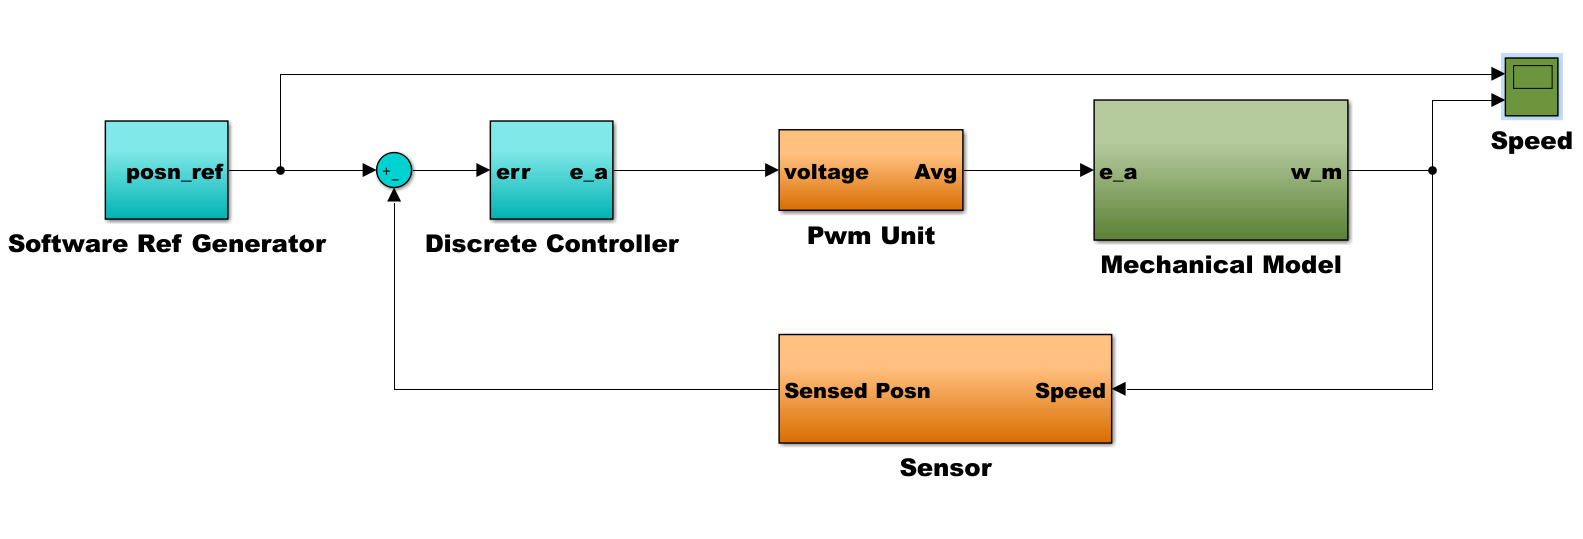
\includegraphics [scale = 0.4] {Figures/Simulink.png}
	\caption{Top level of the dc motor control system}
\end{figure}

% --------------------------------------------- Diagram of Simulink System -------------------------------------------- %

\subsubsection{DC Motors Circuit Diagram}
Figure 4 is a circuit diagram for showing the DC motor drive-train.
\begin{figure} [h!]
	\centering
	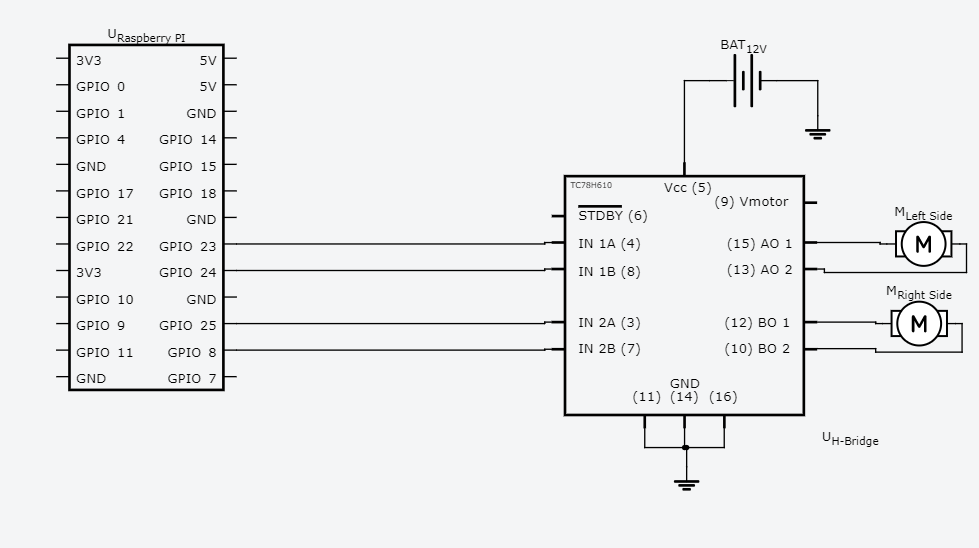
\includegraphics [scale = 0.4] {Figures/H_Bridge.png}
	\caption{H-Bridge Circuit Diagram}
\end{figure}

% --------------------------------------------- DC Motor Specifications -------------------------------------------- %

\subsubsection{DC Motor Specifications}
Manufactured Part Number: 393111-01\\
Rated Voltage: 18V\\
Current: 3A-5A\\

% --------------------------------------------- H-Bridge Specifications -------------------------------------------- %

\subsubsection{H-bridge Specifications}
Manufactured Part Number:  IRF3205\\
Rated Voltage: 3~36V \\
Rated Current: 10A continuous, Peak 30A \\

% --------------------------------------------- Encoder Specifications -------------------------------------------- %

\subsubsection{Encoder Specifications}
Shaft Diameter 6mm\\
Working Range: 3-5V DC\\

% --------------------------------------------- Alfred Pumping System Module -------------------------------------------- %

\subsection{Alfred Pumping System Module}

% --------------------------------------------- Description -------------------------------------------- %

\subsubsection{Description}
This module consists of an Arduino Mega which will receive information from the Alfred manager module through UART to receive the next drink order. This will then begin to dispense the specific drink until it has reached $ m_{containerMin} $. It will then show the customer that the drink has been completed by turning on: $ LED_{drinksignal} $. It will then read $ b_{cuptaken} $ from a light sensor to determine if the cup has been taken at which point it will then wait for the next drink cup to get in place and begin pouring. If it is not able to pump liquid, or it is losing fluid when not dispensing, then it will send the appropriate errors through UART back to the manager.

% --------------------------------------------- Inputs and Outputs -------------------------------------------- %

\subsubsection{Inputs and Outputs}

\textbf{Inputs: } \\

\begin{longtable}{|l|l|l|l|l|}\hline 
		\rowcolor{tableCell}\textbf{Input Name} & \textbf{Input Type} & \textbf{Range} & \textbf{Units} & \textbf{Comment(s)} \\ \hline
		$ b_{cuptaken} $ & Boolean & [0,1] & N/A &  N/A\\ \hline
		\rowcolor{tableCell}$ m_{container} $ & float & [0, 1.0]& Kg & N/A\\ \hline
		$ m_{drink} $    & float & [0, 1.0] & Kg &  N/A\\ \hline
		\rowcolor{tableCell}$ Order_{drinks} $ & Order[] & N/A  & N/A & List of Drinks  \\ \hline
\end{longtable}

\textbf{Outputs: } \\

\begin{longtable}{|l|l|l|l|l|}\hline 
	\rowcolor{tableCell}\textbf{Output Name} & \textbf{Output Type} & \textbf{Range} & \textbf{Units} & \textbf{Comment(s)} \\ \hline
	$ LED_{drinksignal} $ & Boolean & [0,1] & N/A &  N/A\\ \hline
	\rowcolor{tableCell}$ V_{pump } $ & float & [0, 5.0]& V & N/A\\ \hline
	$  errors_{pump} $ & Unsigned Byte & [0, $2^{8}$]& N/A & N/A\\ \hline
\end{longtable}


% ----------------------------------------------------- Exception Handling ---------------------------------------------------- %
\subsubsection{Exception Handling}

\begin{longtable}{|l|l|l|l|}\hline 
		\rowcolor{tableCell}\textbf{Input Name} & \textbf{Input Type} & \textbf{Exception} & \textbf{Exception Handling} \\ \hline
		$ b_{cuptaken} $ & Boolean & N/A &  N/A\\ \hline
		\rowcolor{tableCell}$ m_{container} $ & float & N/A & N/A \\ \hline
		$ m_{drink} $  & float & N/A & N/A \\ \hline
		\rowcolor{tableCell}$ Order_{drinks} $ & Order[] & $ Order_{drinks} $ formatting error & Server Validation \\ \hline
\end{longtable}

% --------------------------------------------- TIming Constraints -------------------------------------------- %

\subsubsection{Timing Constraints}
This module will have to dispense the drink within $ t_{maxpump} $

% --------------------------------------------- Initialization -------------------------------------------- %

\subsubsection{Initialization}
This module start by waiting for the manager to send the drink information for the system to pour. All errors within the system will start as false until they have been triggered.


\pagebreak


% -------------------------------------------- Diagram of DC Pump Control System -------------------------------------------- %

\subsubsection{Diagram of DC Pump Control System}
Figure 5 is a diagram that shows the top level of the dc pump control system. 
\begin{figure} [h!]
	\centering
	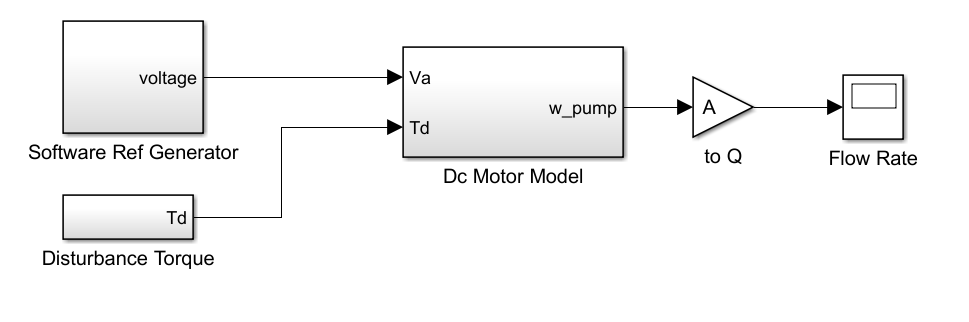
\includegraphics [scale = 0.6] {Figures/DC_PumpSim.png}
	\caption{Top level of the dc motor control system}
\end{figure}


% --------------------------------------------- DC Pump Circuit Diagram -------------------------------------------- %

\subsubsection{DC Pump Circuit Diagram}
Figure 6 is a diagram that shows the DC Pump Circuit.
\begin{figure} [h!]
	\centering
	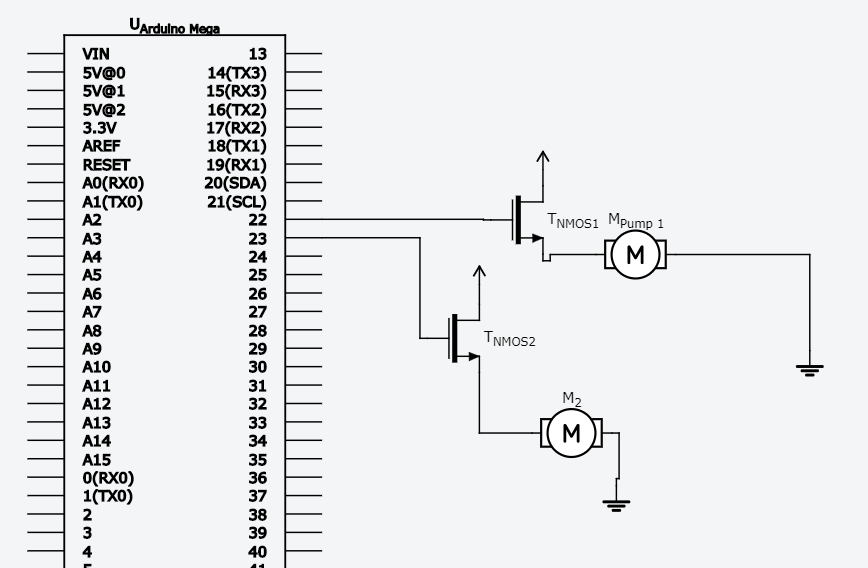
\includegraphics [scale = 0.6] {Figures/Pump.png}
	\caption{DC Pump Circuit Diagram}
\end{figure}


\pagebreak


% --------------------------------------------- Liquid Temperature Circuit Diagram -------------------------------------------- %

\subsubsection{Liquid Temperature Circuit Diagram}
Figure 7 is a circuit diagram for sensing the temperature of the liquid.
\begin{figure} [h!]
	\centering
	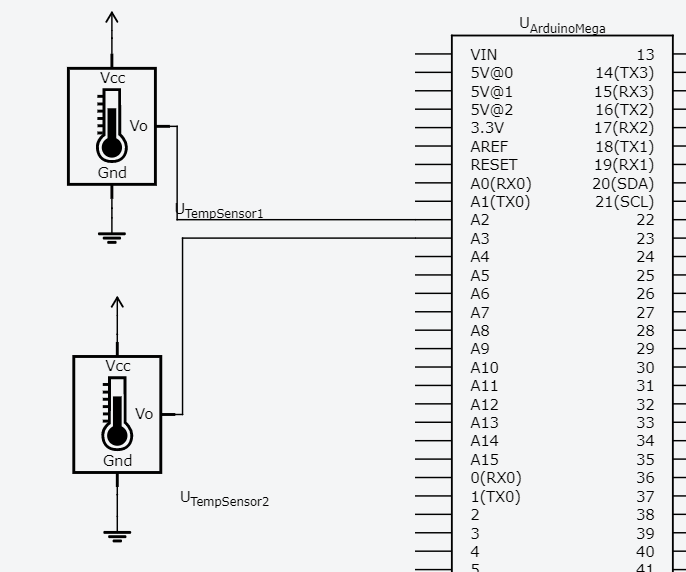
\includegraphics [scale = 0.6] {Figures/TempSensor.png}
	\caption{Top level of the dc motor control system}
\end{figure}

% --------------------------------------------- Weight Detection Circuit Diagram -------------------------------------------- %

\subsubsection{Weight Detection Circuit Diagram}
Figure 8 is a circuit diagram for sensing the weight of the storage containers.
\begin{figure} [h!]
	\centering
	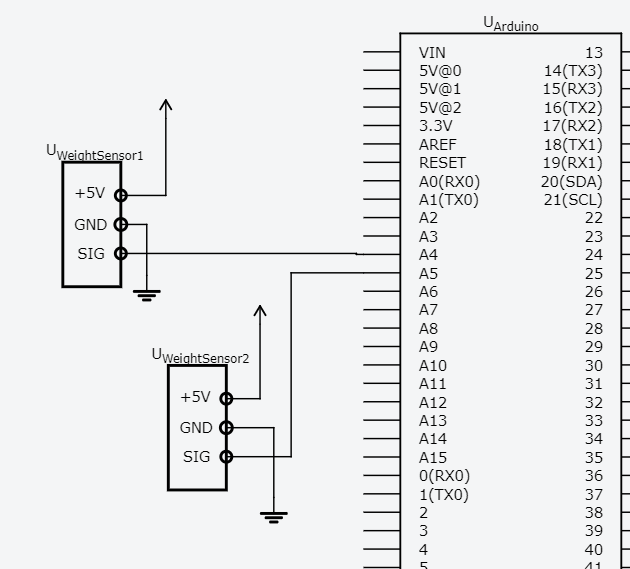
\includegraphics [scale = 0.5] {Figures/WeightSensors.png}
	\caption{Weight Detection Circuit Diagram}
\end{figure}

% --------------------------------------------- DC Pump Specifications -------------------------------------------- %

\subsubsection{DC Pump Specifications}
Manufacture : Yosoo \\
DC Voltage: 3-6V\\
Flow rate: 80-120L/H\\
Material: engineering plastic\\
Diameter: 24.5mm by 46mm \\
Outside diameter:  0.3" 

% --------------------------------------------- Arduino Mega Specifications -------------------------------------------- %

\subsubsection{Arduino Mega Specifications} 
Microcontroller:	ATmega1280\\
Operating Voltage:	5V\\
Digital I/O Pins: 54 (of which 15 provide PWM output)\\
Analog Input Pins: 16\\
DC Current per I/O Pin: 40 mA\\
DC Current for 3.3V Pin: 50 mA\\
Flash Memory: 128 KB\\
Clock Speed: 16MHz\\

% --------------------------------------------- Container Specifications -------------------------------------------- %

\subsubsection{Container Specifications} 

Manufacture : Rubbermaid \\
Dimensions: 10 1/2" x 9" x 4" 
Capacity: 18 Cups/4.2 L\\

% --------------------------------------------- Tubing Specifications -------------------------------------------- %

\subsubsection{Tubing Specifications}
Manufacture : Plumb Craft \\
Diameter: 1/4"ID Food Grade Tubing will be used.\\


% --------------------------------------------- Alfred Image Processing Module -------------------------------------------- %

\subsection{Alfred Image Processing Module }

% --------------------------------------------- Description -------------------------------------------- %

\subsubsection{Description}
This module will receive information from a camera while the drive-train is in motion. This camera will be looking at the ceiling looking for positions of circles that will denote one meter distances set up within a grid around the ceiling of the restaurant. This module will determine if there is a new marker within the image and if so where is the X and Y position of that marker to provide to the drive-train.

% --------------------------------------------- Inputs and Outputs -------------------------------------------- %

\subsubsection{Inputs and Outputs}

\textbf{Inputs: } \\

\begin{longtable}{|l|l|l|l|l|}\hline 
	\rowcolor{tableCell}\textbf{Input Name} & \textbf{Input Type} & \textbf{Range} & \textbf{Units} & \textbf{Comment(s)} \\ \hline
	 $ Image_{input} $ & Bitmap &  N/A & N/A & Image of the ceiling  \\ \hline
\end{longtable}


\pagebreak


\textbf{Outputs: } \\

\begin{longtable}{|l|l|l|l|l|}\hline 
	\rowcolor{tableCell}\textbf{Output Name} & \textbf{Output Type} & \textbf{Range} & \textbf{Units} & \textbf{Comment(s)} \\ \hline
	$ Marker_{PosX} $ & Unsigned Integer & [0,$2^{16}$] & Pixels &  N/A\\ \hline
	\rowcolor{tableCell}$ Marker_{PosY} $ & Unsigned Integer & [0,$2^{16}$] & Pixels & N/A\\ \hline
	$ b_{NextMarkerFound} $ & Boolean & [0,1] & N/A & N/A\\ \hline
\end{longtable}

% ----------------------------------------------------- Exception Handling ---------------------------------------------------- %
\subsubsection{Exception Handling}

\begin{longtable}{|l|l|l|l|l|}\hline 
	\rowcolor{tableCell}\textbf{Input Name} & \textbf{Input Type} & \textbf{Exception} & \textbf{Exception Handling} \\ \hline
	 $ Image_{input} $ & Bitmap &  N/A & N/A \\ \hline
\end{longtable}

% --------------------------------------------- Timing Constraints -------------------------------------------- %

\subsubsection{Timing Constraints}
This information must process in time for the drive train to be able to navigate based off of it.

% --------------------------------------------- Initialization -------------------------------------------- %

\subsubsection{Initialization}
This module start by the drive-train application.

% --------------------------------------------- Raspberry Pi Specifications -------------------------------------------- %

\subsubsection{Raspberry PI Camera Specifications}
Manufacturer: Raspberry PI \\
Resolution: 1080p30, 720p60 and 640 × 480p60/90\\
Field of View (FOV): 62.2 degrees by 48.8 degrees\\


% --------------------------------------------- Modules Likelihood of Change -------------------------------------------- %

\section{Likelihood of Change}

\begin{longtable}{| p{.30\textwidth } | p{.23\textwidth } |  p{.28\textwidth } |}\hline 
\multicolumn{1}{|c|}{\textbf {Module}} & 
\begin{minipage}{.25 \columnwidth}\begin{center}\vspace{1.5mm}\textbf{Likelihood of Change}   \vspace{1.5mm} \end{center}\end{minipage}& 
\multicolumn{1}{c|}{\textbf {Rationale}} \\ \hline

\rowcolor{tableCell} \multicolumn{1}{|c|}{Ordering System Module}& 
\multicolumn{1}{|c|}{Very Unlikely} & Key implementation aspect \\ \hline

\multicolumn{1}{|c|}{Manager Login Page Module}& 
\multicolumn{1}{|c|}{Very Unlikely} & Key implementation aspect \\ \hline

\rowcolor{tableCell} \multicolumn{1}{|c|}{Manager Station Map Software Module}& 
\multicolumn{1}{|c|}{Very Unlikely} & Key implementation aspect \\ \hline

\multicolumn{1}{|c|}{Manager Station Request Software Module}& 
\multicolumn{1}{|c|}{Very Unlikely} & Key implementation aspect \\ \hline

\rowcolor{tableCell} \multicolumn{1}{|c|}{Back End Web Service Module}& 
\multicolumn{1}{|c|}{Very Unlikely} & Key implementation aspect \\ \hline

\multicolumn{1}{|c|}{Alfred Manager Module}& 
\multicolumn{1}{|c|}{Very Unlikely} & Key implementation aspect \\ \hline

\rowcolor{tableCell} \multicolumn{1}{|c|}{Alfred Pumping System Module}& 
\multicolumn{1}{|c|}{Very Unlikely} & Key implementation aspect \\ \hline

\multicolumn{1}{|c|}{Alfred Image Processing Module}& 
\multicolumn{1}{|c|}{Very Unlikely} & Key implementation aspect \\ \hline


\end{longtable}



% --------------------------------------------- Normal Operation -------------------------------------------- %

\section{Normal Operation}
Alfred is a mostly autonomous robot, only requiring human intervention in the event of an error or warning. Alfred will be able to navigate the restaurant by itself, and will serve drinks to tables. Customers will be able to place orders via a mobile application, which will be sent to a server. Orders to serve will be sent to Alfred using a FIFO protocol. Once Alfred has finished with an order, it will be able to request for a new order to serve. Management will be able to recall Alfred to the kitchen at any point using the admin console. In the event of a recall, Alfred will finish the current job and will return to the kitchen afterwards. Management will also be able to create a map of the restaurant and upload it to Alfred, which will give Alfred the means to navigate the restaurant.


% --------------------------------------------- Undesired Event Handling -------------------------------------------- %

\section{Undesired Event Handling}
Alfred will be able to detect undesired behaviours and conditions such as low liquid levels below threshold $ m_{containerMin} $, any issues with pumping liquid, low battery level, leaking liquids, and any blockages in the current path once Alfred has been blocked for a time greater than $ obstruction_{timeout} $. In the event of any error condition, Alfred will send an error code to the kitchen, to alert the staff of the issue. Wherever possible, Alfred will return to the kitchen in an error condition to request a fix. Otherwise, if movement is not possible, the kitchen staff will have to pick Alfred up from the dining room. Along with alerting management of any current errors, Alfred will also be able to indicate whether it is returning to the kitchen or requires pickup.



% ----------------------------------------------------- CLIENT APPLICATION ---------------------------------------------------- %

\section {ClientApp}

% ----------------------------------------------------- Purpose ---------------------------------------------------- %

\subsection{Purpose}
The following will describe the component software design associated with the Client Application. This will be carried out within android based tools to allow customers to order drinks from any table..

% -----------------------------------------------------Scope ---------------------------------------------------- %

\subsection{Scope}
The scope of this section is associated with any front end user interfaces that the customers will use.

% ------------------------------------------- Module Decomposition ------------------------------------------- %

\subsection{Module Decomposition}

\textbf{Activity\_Login}: GUI class for admin to log into client app device.

\textbf{Activity\_Settings}: GUI class for admin to reset device cart, as well as change the table number of the client device. Secrets include parsing and storing table info coming from the server.

\textbf{Activity\_DrinksList [Requirement T01]}: GUI class for users to go through available drinks and choose their order. Secrets include parsing drink info coming from the server.

\textbf{Activity\_OrderCart [Requirement T01]}: GUI class for users to view their current cart, as well as their previous orders. Secrets include parsing and dealing with server's response when order is sent to the server.

\textbf{DrinksViewAdapter}: Adapter class for each visible drink in Activity\_DrinksList

\textbf{DrinkCartListAdapter}: Adapter class for each cart item in Activity\_OrderCart

\textbf{Drink}: Object class representing a drink item.

\textbf{DrinkOrder}: Object class representing a table's order to be sent to the server. 

\textbf{NetworkCalls [Requirement T02]}: Asynchronous class to perform network calls for the client app. Secrets include how network requests/responses are handled.

\textbf{AsyncResponse [Requirement T02]} Interface to deliver NetworkCall results to the current activity for processing.

% ----------------------------------------------------- Uses Relation ---------------------------------------------------- %

\subsection{Uses Relation}

Please refer to Figure 1 on following page.

\begin{figure} [h!]
	\centering
	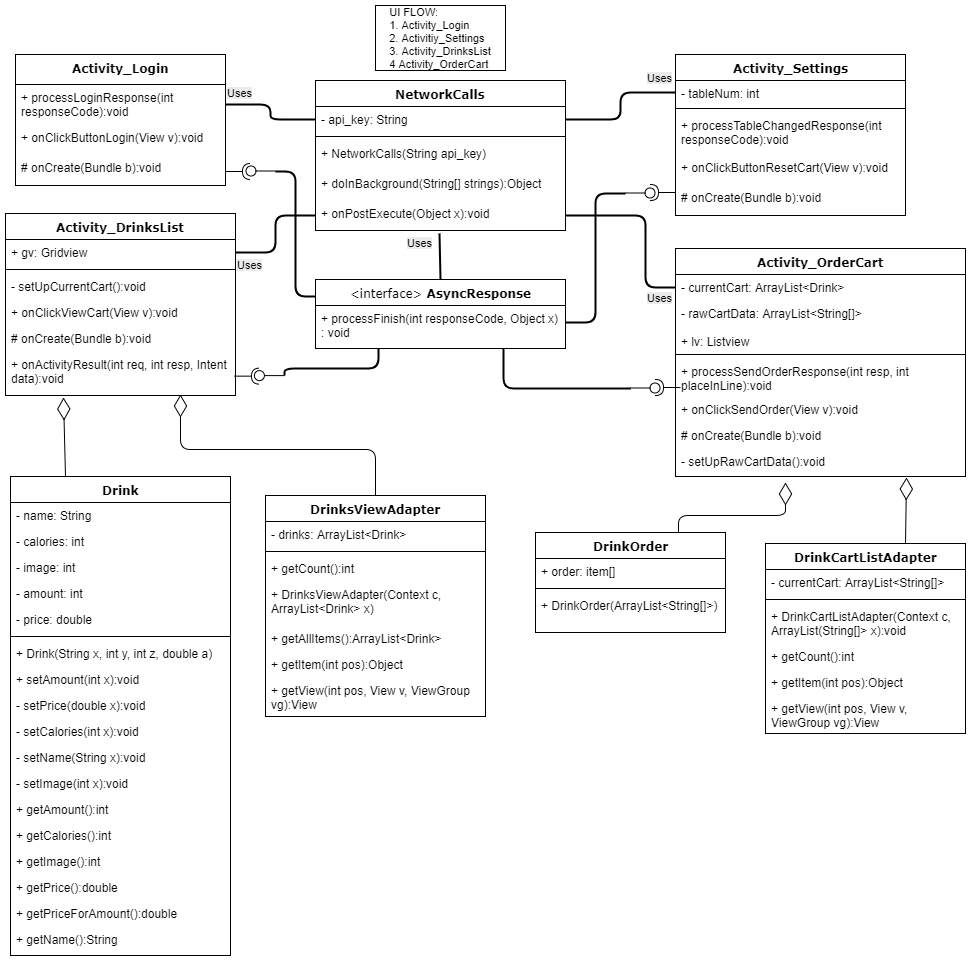
\includegraphics [scale = 0.4] {figures/Client_UsesDiagram.png}
	\caption{Android Client Application Uses Relation Diagram}
\end{figure}



\subsection{MIS}

% ------------------------------------- Drink  ------------------------------------- %

\subsubsection{Drink}

\textbf{Uses} : None

\textbf{Public Functions}

\textbf{Drink(String name,int calories,int image,double price)}
Constructor for Drink class. Takes the name, image, and price of the drink, and the amount of calories in a serving.

\textbf{setAmount(int amt):void}
Sets the number of drinks of this type in the cart.

\textbf{getName():String}
Returns the name of the drink.

\textbf{getCalories():int}
Returns the amount of calories for the restaurant's serving size.

\textbf{getImage():int}
Returns the id number for the image of this drink type.

\textbf{getPrice():double}
Returns the price of this drink.

\textbf{getPriceForAmount():double}
Returns the total price of the amount of this drink.

\textbf{getAmount():int}
Returns the amount of the drink currently in the cart.

% ------------------------------------- Drink Order ------------------------------------- %

\subsubsection{DrinkOrder}

\textbf{Uses} : None

\textbf{Public Functions}

\textbf{DrinkOrder(ArrayList<String[]> rawCartData)}
Constructor for DrinkOrder class. Takes the raw cart data for the currently selected drinks.


\pagebreak 


% ------------------------------------- Activity Drink List  ------------------------------------- %

\subsubsection{Activity\_DrinksList}

\textbf{Uses}

\begin{itemize}
	\item DrinksViewAdapter (Class)
	\item NetworkCalls (Class)
	\item AsyncResponse (Interface)
\end{itemize}

\textbf{onActivityResult(int requestCode, int responseCode, Intent data):void}
Process the results of any activities launched by this activity.

\textbf{onClickViewCart(View v):void}
Listener for the view cart button. Launches Activity\_OrderCart.

\textbf{processDrinksInfoResponse(int responseCode):void}
Processes the response of the drink info retrieval from the server.

\textbf{onCreate(Bundle savedInstanceState):void}
Initialize this Activity(app menu) when created.

% ------------------------------------- Activity/ Login  ------------------------------------- %

\subsubsection{Activity\_Login}

\textbf{Uses}
\begin{itemize}
	\item NetworkCalls (Class)
	\item AsyncResponse (Interface)
\end{itemize}

\textbf{Public Functions}

\textbf{onClickButtonLogin(View v):void}
Listener for the login button. Attempts to log in with filled in username and password.

\textbf{onCreate(Bundle savedInstanceState):void}
Initialize this Activity(app menu) when created.

% ------------------------------------- Activity/ Settings  ------------------------------------- %

\subsubsection{Activity\_Settings}

\textbf{Uses}
\begin{itemize}
	\item NetworkCalls (Class)
	\item AsyncResponse (Interface)
\end{itemize}

\textbf{onClickButtonResetCart(View v):void}
Listener for the reset cart button. Resets the cart for the next guests.

\textbf{processTableChangeResponse(int responseCode, String token):void}
Processes the class specific changes based on the response from the server.

\textbf{onCreate(Bundle savedInstanceState):void}
Initialize this Activity(app menu) when created.

% ------------------------------------- Activity/ Order Cart  ------------------------------------- %

\subsubsection{Activity\_OrderCart}

\textbf{Uses}
\begin{itemize}
	\item DrinkCartListAdapter (Class)
	\item NetworkCalls (Class)
	\item AsyncResponse (Interface)
\end{itemize}

\textbf{Public Functions}

\textbf{processSendOrderResponse(int responseCode, int placeInLine):void}
Processes the response of attempt to place an order with the server.

\textbf{onClickSendOrder(View v):void}
Listener for the send order button. Sends the current cart to the server.

\textbf{onCreate(Bundle savedInstanceState):void}
Initialize this Activity(app menu) when created.

% ------------------------------------- Network Calls  ------------------------------------- %

\subsubsection{NetworkCalls}

\textbf{Uses}
\begin{itemize}
	\item AsyncResponse (Interface)
\end{itemize}


\textbf{Public Functions}

\textbf{NetworkCalls(String api\_key)}
Constructor for NetworkCalls. Takes the api key.

\textbf{doInBackground(String[] strings):Object}
Executes the HTTP request based on the api key provided.

\textbf{onPostExecute(Object result):void}
Processes the response after doInBackground is completed.

\subsubsection{Interface AsyncResponse}
\textbf{Uses} : None

\textbf{Public Functions}

\textbf{processFinish(int responseCode, Object x): void}
Processes data in calling activity after NetworkCalls is completed execution.

% ------------------------------------- Drinks View Adapter ------------------------------------- %

\subsubsection{DrinksViewAdapter}

\textbf{Uses}
\begin{itemize}
	\item Drink (Class)
\end{itemize}

\textbf{Public Functions}

\textbf{DrinksViewAdapter(Context context, ArrayList<Drink> drinks)}
Constructor for DrinksViewAdapter. Takes the context of this adapter and the list of drink info.

\textbf{getCount():int}
Returns the amount of items in the list of drinks.

\textbf{getAllItems():ArrayList<Drink>}
Returns the list of drink info.

\textbf{getItem(int position):Object}
Returns the item for the position id passed to it.

\textbf{getView(int position, View v, ViewGroup parent):View}
Returns the view for the position id passed to it. Takes the position id, current View, and ViewGroup.


% ------------------------------------- Drink Cart List Adapter  ------------------------------------- %

\subsubsection{DrinkCartListAdapter}

\textbf{Uses} None

\textbf{Public Functions}

\textbf{DrinkCartListAdapter(Context context, ArrayList<String[]> currentCartInfo)}
Constructor for DrinkCartListAdapter. Takes the context of this adapter and the current cart information.

\textbf{getCount():int}
Returns the amount of items in the cart.

\textbf{getItem(int position):Object}
Returns the item for the position id passed to it.

\textbf{getView(int position, View v, ViewGroup parent):View}
Returns the view for the position id passed to it. Takes the position id, current View, and ViewGroup.

% --------------------------------------------------------------- MID -------------------------------------------------------------------- %

\subsection{MID}

% ------------------------------------- Drink  ------------------------------------- %

\subsubsection{Drink}

\textbf{Uses} : None

\textbf{Internal Variables}
\textbf{name: String} - Name of the drink

\textbf{calories: int} - Number of calories in a serving of this drink

\textbf{image: int} - id of the image of this drink

\textbf{amount: int} - the amount of this drink currently selected by the user

\textbf{Functions}

\textbf{Drink(String name,int calories,int image,double price)}
Constructor for Drink class. Takes the name, image, and price of the drink, and the amount of calories in a serving. Sets the internal variable values.

\textbf{public setAmount(int amt):void}
Sets the number of drinks of this type in the cart.

\textbf{private setName(String name):void}
Sets the name of the drink. Takes in the name of the drink.

\textbf{private setCalories(int cals):void}
Sets the amount of calories for the restaurant's serving size. Takes in amount of calories.

\textbf{private setImage(int imgID):void}
Sets the id number for the image of this drink type. Takes in an integer image id.

\textbf{private setPrice(double price):void}
Sets the price of this drink. Takes in the price of the drink.

\textbf{public getName():String}
Returns the name of the drink.

\textbf{public getCalories():int}
Returns the amount of calories for the restaurant's serving size.

\textbf{public getImage():int}
Returns the id number for the image of this drink type.

\textbf{public getPrice():double}
Returns the price of this drink.

\textbf{public getAmount():int}
Returns the amount of this drink currently in the cart.

\textbf{public getPriceForAmount():double}
Returns the total price of the amount of this drink.

\subsubsection{DrinkOrder}
\textbf{Uses} : None

\textbf{Internal Variables}

\textbf{order: item[]} - Array of drink items

\textbf{Functions}

\textbf{public DrinkOrder(ArrayList<String[]> rawCartData)}
Constructor for DrinkOrder class. Takes the raw cart data for the currently selected drinks.

% ------------------------------------- Activity/ Drink List------------------------------------- %

\subsubsection{Activity\_DrinksList}

\textbf{Uses}

\begin{itemize}
	\item DrinksViewAdapter (Class)
	\item NetworkCalls (Class)
	\item AsyncResponse (Interface)
\end{itemize}

\textbf{Internal Variables}
\textbf{gv: GridView} - The view holding the list of drink items

\textbf{Functions}

\textbf{public onActivityResult(int requestCode, int responseCode, Intent data):void}
Process the results of any activities launched by this activity.

\textbf{public onClickViewCart(View v):void}
Listener for the view cart button. Launches Activity\_OrderCart.

\textbf{public processDrinksInfoResponse(int responseCode):void}
Processes the response of the drink info retrieval from the server.

\textbf{protected onCreate(Bundle savedInstanceState):void}
Initialize this Activity(app menu) when created. Retrieve the drink info from the server and initialize each item in the gridview as a DrinksViewAdapter. 

\textbf{private setUpCurrentCart():ArrayList<Drink>}
Retrieves and returns the items stored in gv.

% ------------------------------------- Activity/ Login ------------------------------------- %

\subsubsection{Activity\_Login}

\textbf{Uses}

\begin{itemize}
	\item NetworkCalls (Class)
	\item AsyncResponse (Interface)
\end{itemize}

\textbf{Internal Variables} None

\textbf{Functions}
\textbf{public processLoginResponse(int responseCode):void}
Processes class specific changes based on the log in attempt. If (responseCode == 200) then launch settings page. Else show alert.

\textbf{public onClickButtonLogin(View v):void}
Listener for the login button. Attempts to log in with filled in username and password. Executes a NetworkCall task with the correct api key passed.

\textbf{protected onCreate(Bundle savedInstanceState):void}
Initialize this Activity(app menu) when created.

% ------------------------------------- Activity/ Settings ------------------------------------- %

\subsubsection{Activity\_Settings}

\textbf{Uses}
\begin{itemize}
	\item NetworkCalls (Class)
	\item AsyncResponse (Interface)
\end{itemize}

\textbf{Internal Variables}
\textbf{tableNum: int} - The table number associated with this device.

\textbf{Functions}
\textbf{public onClickButtonResetCart(View v):void}
Listener for the reset cart button. Resets the cart for the next guests. Clears all cart information.

\textbf{public processTableChangeResponse(int responseCode, String token):void}
Processes the class specific changes based on the response from the server. If (responseCode == 200) then store the token and new tableNum. Else show alert and keep tableNum the same.

\textbf{onCreate(Bundle savedInstanceState):void}
Initialize this Activity(app menu) when created.

% ------------------------------------- Activity/ Order Cart ------------------------------------- %

\subsubsection{Activity\_OrderCart}

\textbf{Uses}

\begin{itemize}
	\item DrinkCartListAdapter (Class)
	\item NetworkCalls (Class)
	\item AsyncResponse (Interface)
\end{itemize}

\textbf{Internal Variables}
\textbf{currentCart: ArrayList<Drink>} - ArrayList of Drink objects representing the current cart selections.

\textbf{rawCartData: ArrayList<String[]>} - ArrayList of String[] representing the current cart. This is data used for the DrinkCartListAdapter.

\textbf{lv: ListView} - The view which contains and displays the cart items.

\textbf{Functions}
\textbf{public processSendOrderResponse(int responseCode, int placeInLine):void}
Processes the response of attempt to place an order with the server.

\textbf{public onClickSendOrder(View v):void}
Listener for the send order button. Sends the current cart to the server.

\textbf{protected onCreate(Bundle savedInstanceState):void}
Initialize this Activity(app menu) when created.

\textbf{private setUpRawCartData():void}
Uses the information from the currentCart to set up an ArrayList<String[]>. Each item in the ArrayList is a String array consisting of [name, amount, price for amount]

% ------------------------------------- Network Calls ------------------------------------- %

\subsubsection{NetworkCalls}

\textbf{Uses}
\begin{itemize}
	\item AsyncResponse (Interface)
\end{itemize}
\textbf{Internal Variables}

\textbf{api\_key: String} - String representing the api being targeted. Used for conditionals.

\begin{itemize}
	\item "table\_token" - target (HOST)$\backslash$table?tableId=?
	\item "placeOrder" - target (HOST)$\backslash$placeOrder?tableId=?
	\item "login" - target (HOST)$\backslash$login
\end{itemize}

\textbf{Functions}

\textbf{public NetworkCalls(String api\_key)}
Constructor for NetworkCalls. Takes the api key.

\textbf{public doInBackground(String[] strings):Object}
Executes the HTTP request based on the api key provided.

\textbf{public onPostExecute(Object result):void}
Processes the response after doInBackground is completed.

% ------------------------------------- Interface Async Response ------------------------------------- %

\subsubsection{Interface AsyncResponse}

\textbf{Uses}:None

\textbf{Internal Variables} : None

\textbf{Functions}

\textbf{public processFinish(int responseCode, Object x): void}
Processes data in calling activity after NetworkCalls is completed execution.

% ------------------------------------- Drink View Adapter ------------------------------------- %

\subsubsection{DrinksViewAdapter}

\textbf{Uses}

\begin{itemize}
	\item Drink (Class)
\end{itemize}

\textbf{Internal Variables}

\textbf{drinks: ArrayList<Drink>} - ArrayList of Drink objects representing the current cart selections.

\textbf{Functions}

\textbf{public DrinksViewAdapter(Context context, ArrayList<Drink> drinks)}
Constructor for DrinksViewAdapter. Takes the context of this adapter and the list of drink info.

\textbf{public getCount():int}
Returns the amount of items in the list of drinks.

\textbf{public getAllItems():ArrayList<Drink>}
Returns the list of drink info.

\textbf{public getItem(int position):Object}
Returns the item for the position id passed to it.

\textbf{public getView(int position, View v, ViewGroup parent):View}
Returns the view for the position id passed to it. Takes the position id, current View, and ViewGroup.

% ------------------------------------- Drink Cart List Adapter ------------------------------------- %

\subsubsection{DrinkCartListAdapter}

\textbf{Uses} None

\textbf{Internal Variables}
\textbf{currentCart: ArrayList<String[]>} - ArrayList of Drink objects representing the current cart selections.

\textbf{Functions}
\textbf{public DrinkCartListAdapter(Context context, ArrayList<String[]> currentCartInfo)}
Constructor for DrinkCartListAdapter. Takes the context of this adapter and the current cart information.

\textbf{public getCount():int}
Returns the amount of items in the cart.

\textbf{public getItem(int position):Object}
Returns the item for the position id passed to it.

\textbf{public getView(int position, View v, ViewGroup parent):View}
Returns the view for the position id passed to it. Takes the position id, current View, and ViewGroup.


\pagebreak


% ------------------------------------------------------ MANAGER SYSTEM ----------------------------------------------------- %

\section {Manager System}

% ------------------------------------------------ Purpose --------------------------------------------- %

\subsection{Purpose}
The following will describe the component software design associated with Manager System. This will be carried out within web based tools to allow management to access there information anywhere.

% ------------------------------------------------ Scope --------------------------------------------- %

\subsection{Scope}

The scope of this section is associated with any front end user interfaces that the management staff will use. This includes the MIS/MID and uses relation in regards to the Map Making Page, the Error Viewing page and the Login System. 

% --------------------------------------- Module Decomposition ------------------------------------- %

\subsection{Module Decomposition}

\textbf{Manager Login Page}: Given the login credentials, will authenticate administrator of the system with the server. Secrets include how it goes about verifying with the server if the credentials are valid.
\textbf{Manager Station Map Software Page}: Will allow administrator to create or modify the map of the area where Alfred will deliver drinks. This map will then be sent and stored on the server. The secrets of this module includes how the mapping system will translate user input into the map file
\textbf{Manager Station Request Software Page}: Will allow administrator to execute commands for Alfred, as well as view incoming error codes from Alfred. Secrets include how the errors are decoded from the server.

% ----------------------------------------------- Uses Relation ------------------------------------------- %

\subsection{Uses Relation}

\begin{figure} [h!]
	\centering
	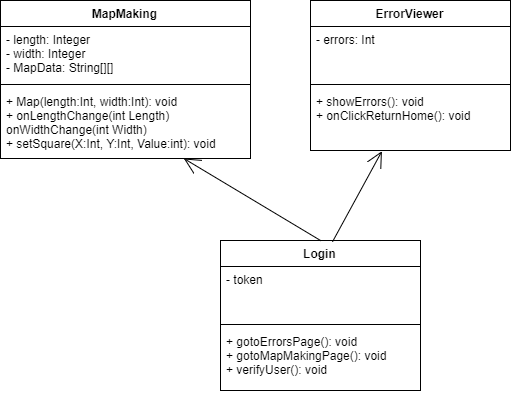
\includegraphics [scale = 0.4] {figures/Manager_UsesDiagram.png}
	\caption{Alfred Uses Relation Diagram}
\end{figure}


% ------------------------------------------------------- MIS ----------------------------------------------------- %

\subsection{MIS}

% ------------------------------------ Login Page ------------------------------------ %

\subsubsection{Login Page}

\textbf{Uses}
\begin{itemize}
	\item MapMaking (WebPage)
	\item ErrorViewer (WebPage)
\end{itemize}


\pagebreak 


\textbf{Public Functions}

\textbf{gotoErrorsPage(): void}
Navigates to the page associated with showing the Managers page for Errors with Alfred.

\textbf{gotoMapMakingPage(): void}
Navigates to the page associated with showing the Managers page for creating a resturant Map.

\textbf{verifyUser(): void}
Determines if the information that the user put into the form on the webpage is correct.

% ------------------------------ Map Making Page ------------------------------- %

\subsubsection{MapMaking Page}
\textbf{Uses}
None

\textbf{Public Functions}

\textbf{ Map(length:Int, width:Int): void}
Constructor to object for page load

\textbf{onLengthChange(int Length)}
Sets the length of the map when the user changes it in the form. This is based on requirement AD1.

\textbf{onWidthChange(int Width)}
Sets the width of the map when the user changes it in the form.This is based on requirement AD1.

\textbf{setSquare(X:Int, Y:Int, value:Int): void}
Sets the value of the square based on its X,Y position when there is an on click event. This is based on requirement AD2.

% ------------------------------------ Error View Page ------------------------------------ %

\subsubsection{ErrorViewer Page}

\textbf{Uses}
None

\textbf{Public Functions}

\textbf{ showErrors(): void}
Shows the Errors Associated to Alfred. Based on requirement NFR26.
\textbf{onClickReturnHome()}
Signals the Robot to return home. Based on requirement NFR11.


% ------------------------------------------------------- MID ----------------------------------------------------- %

\subsection{MID}

% ------------------------------------  Login Page ------------------------------------ %

\subsubsection{Login Page}

\textbf{Uses}
\begin{itemize}
	\item MapMaking (WebPage)
	\item ErrorViewer (WebPage)
\end{itemize}


\textbf{Internal Variables}

\textbf{token: String} - Token for a session with the server.


\textbf{Functions}

\textbf{public gotoErrorsPage(): void}
Navigates to the page associated with showing the Managers page for Errors with Alfred.

\textbf{public gotoMapMakingPage(): void}
Navigates to the page associated with showing the Managers page for creating a resturant Map.

\textbf{public verifyUser(): void}
Determines if the information that the user put into the form on the webpage is correct.

% ------------------------------------ Map Making Page ------------------------------------ %

\subsubsection{MapMaking Page}

\textbf{Uses}
None

\textbf{Internal Variables}

\textbf{length: Integer} - Length of the Map

\textbf{width: Integer} - Width of the Map

\textbf{MapData: String[][]}- Storage of the map values

\textbf{Public Functions}

\textbf{public Map(length:Int, width:Int): void}

Constructor to object for page load

\textbf{public onLengthChange(int Length)}

Sets the length of the map when the user changes it in the form.

\textbf{public onWidthChange(int Width)}

Sets the width of the map when the user changes it in the form.

\textbf{setSquare(X:Int, Y:Int, value:Int): void}

Sets the value of the square based on its X,Y position when there is an on click event. The Values corresponds to: 
 
\begin{itemize}
	\item 0: Free to move
	\item 1: Path is blocked
	\item 2: Table
	\item 3: Base
\end{itemize}

% ------------------------------------ Error View Page ------------------------------------ %

\subsubsection{ErrorViewer Page}
\textbf{Uses}
None

\textbf{Public Functions}

\textbf{ showErrors(): void}
Shows the Errors Associated to Alfred. where the Errors are in the following format
\begin{itemize}
	\item LowLiquid: 0x00000001
	\item LeakingTank: 0x00000010
	\item LowBattery: 0x00000100
	\item NoMovement: 0x00001000
\end{itemize}

\textbf{onClickReturnHome()}
Signals the Robot to return home.

% ------------------------------------------------------- ALFRED SYSTEM ----------------------------------------------------- %


\section {Alfred System}

% ------------------------------------------------ Purpose ----------------------------------------------- %

\subsection{Purpose}
The following will describe the component software, mechanical and electrical design associated with Alfred's Manager System, Alfred's Drivetrain and Alfred's Image Processing system. These three systems will be ran on the Raspberry Pi. 

% ----------------------------------------------- Scope ------------------------------------------------- %

\subsection{Scope}

The scope of this section is associated with Alfred's Manager System, Alfred's Drivetrain and Alfred's Image Processing system. The software documentation will provide the MIS and MID, uses relations to describe how the system will be designed to preform its function of being able to drive to a specific location. The mechanical and electrical design will focus on the aspects to provide motion and navigation.

% ---------------------------------- Module Decomposition -------------------------------------- %

\subsection{Module Decomposition}

\textbf{Alfred Manager Module}: Endpoint for communication with Alfred. Will manage communication with server, as well as send any errors that Alfred is experiencing. Secrets include Parsing of messages from the server and the pumping system. 
\textbf{Alfred Drive Train Module}: Responsible for driving and managing the motors based on desired route. Will also be sending errors preventing movement to Alfred Manager Module. Secrets include how the robot will preform navigation based on the map, how the robot will control and drive the robot and the inputs from the image processing module.
\textbf{Image Processing Module}: Will detect any obstacles in the way as well as locate incoming nodes. Will communicate with Alfred Drive Train Module, to determine whether any required action based on results. Secretes include how the image processing will be carried out

% ------------------------------------------ Uses Relation -------------------------------------- %

\subsection{Uses Relation}
\begin{figure} [h!]
	\centering
	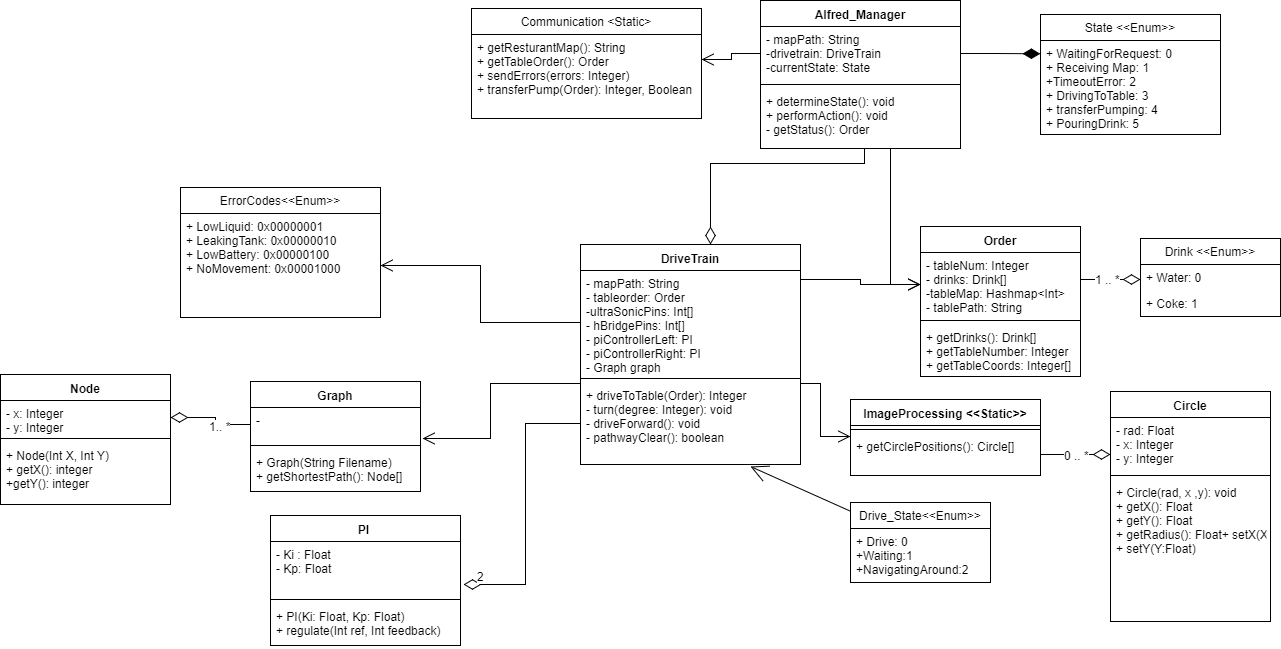
\includegraphics [scale = 0.38] {figures/Alfred_UsesDiagram.png}
	\caption{Alfred Uses Relation Diagram}
\end{figure}

% ------------------------------------------------------- MIS ----------------------------------------------------- %

\subsection{MIS}

% ------------------------ Alfred Manager Class ------------------------------ %

\subsubsection{Alfred Manager Class}

\textbf{Uses}
\begin{itemize}
	\item Communication (Static Class)
	\item State (Enum)
	\item Drivetrain (Class)
	\item Order (Class)
\end{itemize}

\textbf{Public Functions}

\textbf{determineState(): void}

Determines the overall state of Alfred based on the inputs to Alfred. 

\textbf{performAction(): void}

Will preform the desired state based on the state of Alfred.

% ------------------------ Order Class ------------------------------ %

\subsubsection{Order Class}
\textbf{Uses}
\begin{itemize}
	\item Drink (Enum)
\end{itemize}

\textbf{Public Functions}

\textbf{getDrinks()}

Drink[] - Returns the list of drinks. Based on requirement AF1.

\textbf{getTableNumber}

 Integer - Returns the table number reference. Based on requirement AF3.

\textbf{getTableCoords}

 Integer[] - Returns the coordinates to the table. Based on requirement AF3.

% ------------------------ Drivetrain Class ------------------------------ %

\subsubsection{Drivetrain Class}
\textbf{Uses}
\begin{itemize}
	\item Order (Class)
	\item ImageProcessing (Class)
	\item Drive\_State (Enum)
	\item ErrorCodes (Enum)
	\item Circle (Class)
	\item Graph (Class)
	\item Node (Class)
	\item PI (Class)
\end{itemize}

\textbf{Public Functions}
\textbf{driveToTable(Order): Integer}
This function will preform the driving operation in order to navigate towards the specific table. Based on requirement AF3.

% ------------------------ Communication Static Class ------------------------------ %

\subsubsection{Communication Static Class}
\textbf{Uses}

None 

\textbf{Public Functions}

\textbf{getResturantMap(): String}

Retrieves and stores the map to be used for navigation. Returns the path of the map. Based on requirement AF3.

\textbf{getTableOrder(): Order}

Retrieves and returns the Table's Order. Based on requirement AF3.

\textbf{sendErrors(errors: Integer)}

Sends an integer with the described set of integers. Based on requirement NFR26.

\textbf{transferPump(Order): Integer}

Preforms communication with the pumping system. Sends the Order data and receives the errors from the pumping system and if it complete. Based on requirement AF1.

% ------------------------ Graph Class ------------------------------ %

\subsubsection{Graph Class}
\textbf{Uses}
\begin{itemize}
	\item Node (Class)
\end{itemize}

\textbf{Public Functions}

\textbf{Graph(String Filename)}

Constructor to create a graph object. Builds the graph based on the path to the map. Based on requirement AF3.

\textbf{getShortestPath(): Node[]}

Returns a list of nodes that describes the shortest way to get to the destination. 

% ------------------------ Node Class ------------------------------ %

\subsubsection{Node Class}
\textbf{Uses}
None 

\textbf{Public Functions}

\textbf{Node(Int X, Int Y)}

Constructor to the node class, takes in the position of the point along the X Y plane.

\textbf{getX(): integer}


Returns the x coordinate of the node

\textbf{getY(): integer}

Returns the y coordinate of the node

% ------------------------ PI Class ------------------------------ %

\subsubsection{PI Class}
\textbf{Uses}
None 

\textbf{Public Functions}

\textbf{PI(Ki: Float, Kp: Float)}

Constructor for the PI controller object taking in the Ki and Kp terms

\textbf{regulate(Int ref, Int feedback)}

Based on the reference to control to and the feedback, will determine the value to set the outputs too.  Based on requirement AF3 to allow regulated movement to the location.

% ------------------------ Image Processing Static Class ------------------------------ %

\subsubsection{Imaging Processing Static Class}
\textbf{Uses}
\begin{itemize}
	\item Circle (Class)
\end{itemize}

\textbf{Public Functions}

\textbf{getCirclePositions(): Circle[]}

Gives a list of circles that were within the view of the camera

% ------------------------ Circle Class ------------------------------ %

\subsubsection{Circle Class}

\textbf{Uses}
None

\textbf{Public Functions}

\textbf{Circle(radius, x, y)}

Constructor of the circle class, takes in initial radius, x and y values. Based on requirement AF3 to allow regulated movement to the location.

\textbf{getX(): Float}

Gives the X position of the circle relative to the image

\textbf{getY(): Float}

Gives the Y position of the circle relative to the image

\textbf{getRadius(): Float}

Gives the radius of the circle

\textbf{setX(X:Float)}

Sets the X position of the circle.

\textbf{setY(Y:Float)}

Sets the Y position of the circle.

\textbf{setRadius(rad : Float)}

Sets the radius of the circle


% ------------------------------------------------------- MID ----------------------------------------------------- %

\subsection{MID}

% ------------------------ Alfred Manager Class ------------------------------ %

\subsubsection{Alfred Manager Class}

\textbf{Uses}
\begin{itemize}
	\item Communication (Static Class)
	\item State (Enum)
	\item Drivetrain (Class)
	\item Order (Class)
\end{itemize}

\textbf{Internal Variables}

\textbf{mapPath: String} - The absolute path to the map directory

\textbf{drivetrain: DriveTrain} - An object encapsulates information in regards to the drivetrain

\textbf{currentState: State} - Holds the information in regards to which action will be preformed by Alfred


\textbf{Functions}

\textbf{public determineState(): void}

Determines the overall state of Alfred based on the inputs to Alfred based on the following tabular expression:
\begin{figure} [h!]
	\centering
	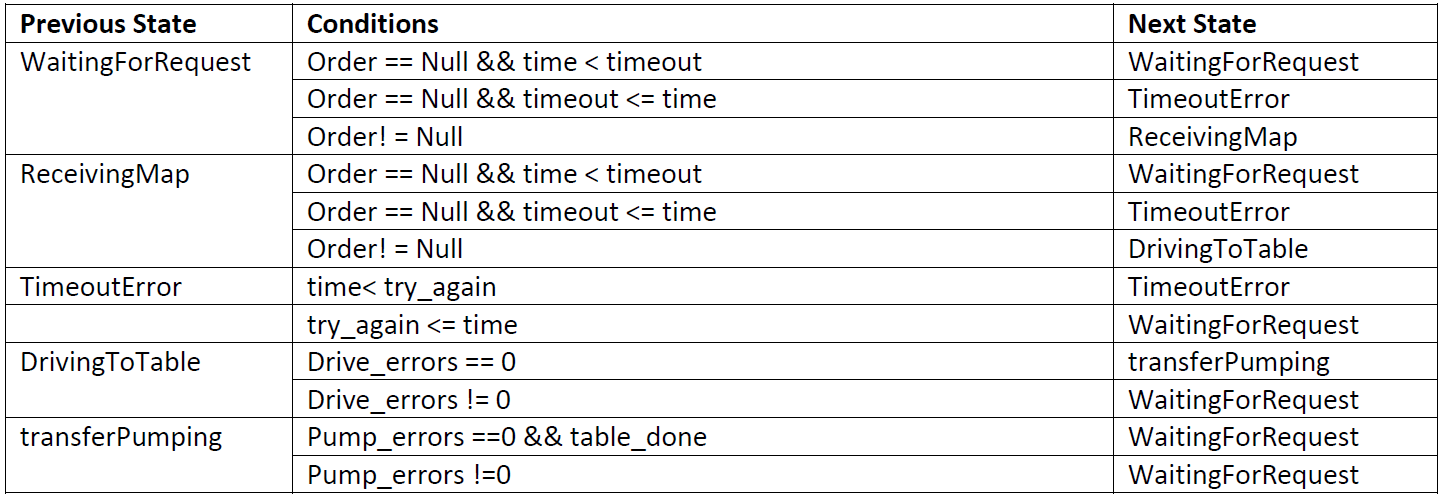
\includegraphics [scale = 0.4] {figures/AlfredSystem_DetermineState.png}
\end{figure}


\textbf{public performAction(): void}

Will preform the desired state based on the state of Alfred based on the following table:
\begin{figure} [h!]
	\centering
	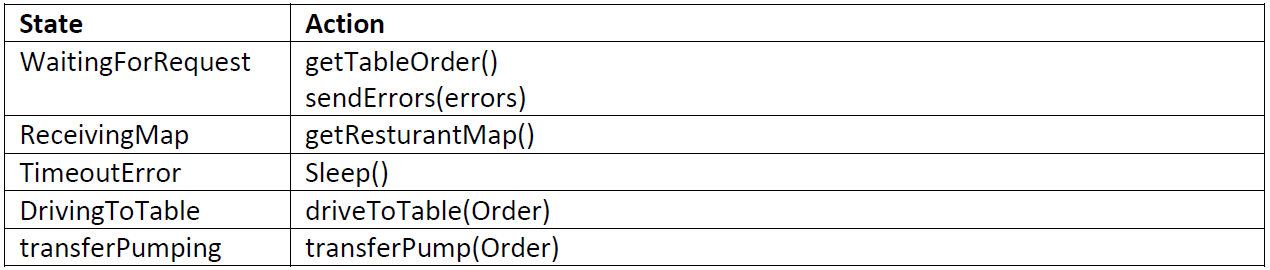
\includegraphics [scale = 0.4] {figures/AlfredSystem_PerformAction.png}
\end{figure}
\subsubsection{Order Class}
\textbf{Uses}
\begin{itemize}
	\item Drink (Enum)
\end{itemize}


\textbf{Internal Variables}

\textbf{tableNum: Integer} - the reference to the table

\textbf{drinks: Drink[]} - List of drinks for the user's table

\textbf{tableMap: Hashmap<Int>} -  Map that takes in a table reference number and returns its X,Y Coord

\textbf{tablePath: String} - gives the path of the table for the hashmap 

\textbf{Functions}

\textbf{public getDrinks(): Drink[]}

Returns the list of drinks

\textbf{public getTableNumber: Integer}

Returns the table number reference

\textbf{public getTableCoords: Integer[]}

Returns the coordinates to the table from the Hashmap of table numbers


% ------------------------ Drivetrain Class ------------------------------ %

\subsubsection{Drivetrain Class}
\textbf{Uses}
\begin{itemize}
	\item Order (Class)
	\item ImageProcessing (Class)
	\item Drive\_State (Enum)
	\item ErrorCodes (Enum)
	\item Circle (Class)
	\item Graph (Class)
	\item Node (Class)
	\item PI (Class)
\end{itemize}


\textbf{Internal Variables}
\textbf{mapPath: String} - The absolute path to the map directory

\textbf{tableorder: Order} - The order from the next table.

\textbf{ultraSonicPins: Int[]} - The pins dedicated for the ultrasonic sensors

\textbf{hBridgePins: Int[]} - The pins dedicated for the H-bridge

\textbf{graph: Graph} - Object to the graph object to find the shortest path

\textbf{piControllerLeft: PI} - Object used for PI control for the left side of the drivetrain

\textbf{piControllerRight: PI} - Object used for PI control for the left side of the drivetrain

\textbf{Functions}

\textbf{public driveToTable(Order): Integer}

This function will preform the driving operation in order to navigate towards the specific table.

\textbf{private turn(degree: Integer): void}

This function will turn relative to its current position the amount desired within the argument. The robot will use the references of the circles to help with alignment by knowing that every node is 90 degrees from one another.

\textbf{private driveForward(void): void}

This function will control the robot to move forward provided: $ \forall front ultrasonic sensors: d_{ultrasonic} > d_{min} $. This motion will use the PI regulators to provide motion at human speed and will continue until a the next circle is within the middle of the camera.

\textbf{private pathwayClear (void): boolean}

This function will determine if robot to move forward provided: $ \forall front ultrasonic sensors: d_{ultrasonic} > d_{min} $. 

\subsubsection{Communication Static Class}
\textbf{Uses}
None 
\textbf{Internal Variables}

None 

\textbf{Functions}

\textbf{getResturantMap(): String}

Retrieves the map file based off of an FTP protocol and stores the map to be used for navigation. Returns the path of the map.

\textbf{getTableOrder(): Order}

Retrieves and returns the Table's Order.

\textbf{sendErrors(errors: Integer)}

 Sends an integer with the described set of integers. 
 
\textbf{transferPump(Order): Integer}

 Performs communication with the pumping system using UART communication. The first 32 bits are the error code of the pumping system and the last bit is the status of the pumping system. Sends the Order data and receives the errors from the pumping system.

% ------------------------ Graph Class ------------------------------ %

\subsubsection{Graph Class}
\textbf{Uses}
\begin{itemize}
	\item Node (Class)
\end{itemize}

\textbf{Internal Variables}
None 

\textbf{Functions}

\textbf{Graph(String Filename)}

Constructor to create a graph object. Builds the graph based on the path to the map

\textbf{getShortestPath(): Node[]}

Returns a list of nodes that describes the shortest way to get to the destination.  The shortest path will be preformed using the map and Dijkstra's algorithm.

% ------------------------ Node Class ------------------------------ %

\subsubsection{Node Class}

\textbf{Uses}
None 

\textbf{Public Functions}

\textbf{Node(Int X, Int Y)}

Constructor to the node class, takes in the position of the point along the X Y plane.

\textbf{getX(): integer}

Returns the x coordinate of the node.

\textbf{getY(): integer}

Returns the y coordinate of the node.

\textbf{Internal Variables}

\textbf{x: Integer} - The x coordinate of the node

\textbf{y: Integer} - The y coordinate of the node

\textbf{Functions}

\textbf{public Node(Int X, Int Y)}

Constructor to the node class, takes in the position of the point along the X Y plane.

\textbf{public getX(): integer}

Returns the x coordinate of the node

\textbf{public getY(): integer}

Returns the y coordinate of the node

% ------------------------ PI Class ------------------------------ %

\subsubsection{PI Class}
\textbf{Uses}
None 
\textbf{Internal Variables}
\textbf{Ki: Float} - Integral temp for the PI controller
\textbf{Kp: Float} - The y coordinate of the node.

\textbf{Functions}

\textbf{public PI(Ki: Float, Kp: Float)}

Constructor for the PI controller object taking in the Ki and Kp terms

\textbf{public regulate(Int ref, Int feedback)}

Based on the reference to control to and the feedback, will determine the value to set the outputs too. Determines the output based along the following formula: $ out = Kp*error+Ki*\int_{0}^{t}(error)dt$. Note that the derivative term is not used due to the error associated with derivatives within computing systems.

% ------------------------ Image Processing Class ------------------------------ %

\subsubsection{Imaging Processing Static Class}

\textbf{Uses}
\begin{itemize}
	\item Circle (Class)
	\item Open CV (External Library)
\end{itemize}

\textbf{Internal Variables}
None

\textbf{Functions}

\textbf{Public getCirclePositions(): Circle[]}

Gives a list of circles that were within the view of the camera. Open CV returns a list of objects which can then be checked to see if they are black circles.

% ------------------------ Circle Class ------------------------------ %

\subsubsection{Circle Class}

\textbf{Uses}
None
\textbf{Internal Variables}

\textbf{rad: Float} - The radius of the circle

\textbf{x: Integer} - The X position of the circle relative to the image

\textbf{y: Integer} - The Y position of the circle relative to the image 

\textbf{Functions}

\textbf{Circle(radius, x, y)}

Constructor of the circle class, takes in initial radius, x and y values

\textbf{getX(): Float}

Gives the X position of the circle relative to the image

\textbf{getY(): Float}

Gives the Y position of the circle relative to the image

\textbf{getRadius(): Float}

Gives the radius of the circle

\textbf{setX(X:Float)}

Sets the X position of the circle.

\textbf{setY(Y:Float)}

Sets the Y position of the circle.

\textbf{setRadius(rad : Float)}

Sets the radius of the circle.

% ------------------------ Raspberry Pi Pin Information ------------------------------ %

\subsubsection{Raspberry Pi Pin Information}
\resizebox{\textwidth}{!}{%
	\begin{tabular}{|l|l|l|l|l|}
		\hline
		From                      & PIN \# (physical) & GPIO \# (BCM) & To                                     & Comments                                                                                                                                                                         \\ \hline
		Raspberry Pi GND GPIO     & 6                 & -             & H-Bridge GND                           & Ground for Motor controller                                                                                                                                                      \\ \hline
		Raspberry Pi 5V GPIO      & 4                 & -             & H-Bridge PWR                           & \begin{tabular}[c]{@{}l@{}}5V supply to H-bridge\\   ***can utilize the 5v pin of the ultrasonic sensors instead of a new pin\end{tabular}                                       \\ \hline
		Raspberry Pi GPIO         & 12                & 18            & H-Bridge DIR 1                         & Direction of motor 1                                                                                                                                                             \\ \hline
		Raspberry Pi GPIO         & 16                & 23            & H-Bridge PWM 1                         & PWM of motor 1                                                                                                                                                                   \\ \hline
		Raspberry Pi GPIO         & 18                & 24            & H-Bridge DIR 2                         & Direction of motor 2                                                                                                                                                             \\ \hline
		Raspberry Pi GPIO         & 22                & 25            & H-Bridge PWM 2                         & PWM of motor 2                                                                                                                                                                   \\ \hline
		Raspberry Pi GND GPIO     & 14                & -             & Ultra sonic sensors GND                & \begin{tabular}[c]{@{}l@{}}Ground for all ultra sonic sensors\\   ***can utilize GND from H-Bridge GND pin\end{tabular}                                                          \\ \hline
		Raspberry Pi 5V GPIO      & 2                 & -             & Ultra sonic sensors VCC                & \begin{tabular}[c]{@{}l@{}}5V supply for all ultrasonic sensors, connected parallel\\   ***can utilize the 5v pin of the H-bridge supply instead of using a new pin\end{tabular} \\ \hline
		Raspberry Pi GPIO         & 24                & 8             & Ultra sonic sensor \#1 TRIG            & Send trigger signal                                                                                                                                                              \\ \hline
		Raspberry Pi GPIO         & 26                & 7             & Ultra sonic sensor \#1 ECHO            &                                                                                                                                                                                  \\ \hline
		Raspberry Pi GPIO         & 3                 & 2             & Ultra sonic sensor \#2 TRIG            & Send trigger signal                                                                                                                                                              \\ \hline
		Raspberry Pi GPIO         & 5                 & 3             & Ultra sonic sensor \#2 ECHO            &                                                                                                                                                                                  \\ \hline
		Raspberry Pi GPIO         & 7                 & 4             & Ultra sonic sensor \#3 TRIG            & Send trigger signal                                                                                                                                                              \\ \hline
		Raspberry Pi GPIO         & 11                & 17            & Ultra sonic sensor \#3 ECHO            &                                                                                                                                                                                  \\ \hline
		Raspberry Pi GND GPIO     & 20                & -             & Encoders GND                           & \begin{tabular}[c]{@{}l@{}}Shared between encoders \\   ***can utilize ultra sonic sensors' GND or H-Bridge GND instead of taking new\\   pin\end{tabular}                       \\ \hline
		Raspberry Pi 3.3V GPIO    & 1                 & -             & Encoders VCC                           & \begin{tabular}[c]{@{}l@{}}Shared between encoders in parallel\\   ***can utilize 5V from either H-Bridge pin or ultra sonic sensors' pin\\   instead of 3.3v\end{tabular}       \\ \hline
		Raspberry Pi GPIO         & 13                & 27            & Encoder \#1 DT                         &                                                                                                                                                                                  \\ \hline
		Raspberry Pi GPIO         & 15                & 22            & Encoder \#1 CLK                        &                                                                                                                                                                                  \\ \hline
		Raspberry Pi GPIO         & 19                & 10            & Encoder \#2 DT                         &                                                                                                                                                                                  \\ \hline
		Raspberry Pi GPIO         & 21                & 9             & Encoder \#2 CLK                        &                                                                                                                                                                                  \\ \hline
		Raspberry Pi GPIO         & 8                 & 14            & Arduino                                & Communication between Arduino and Pi                                                                                                                                             \\ \hline
		Raspberry Pi GPIO         & 10                & 15            & Arduino                                & Communication between Arduino and Pi                                                                                                                                             \\ \hline
		36V Positive terminal     & -                 & -             & H-Bridge power                         & Power supply to motors                                                                                                                                                           \\ \hline
		36V Negative terminal     & -                 & -             & H-Bridge ground                        & Motor ground                                                                                                                                                                     \\ \hline
		Motor 1 positive terminal & -                 & -             & H-Bridge Motor 1 +                     & Positive connection to controller                                                                                                                                                \\ \hline
		Motor 1 negative terminal & -                 & -             & H-Bridge Motor 1 -                     & Negative connection to controller                                                                                                                                                \\ \hline
		Motor 2 positive terminal & -                 & -             & H-Bridge Motor 2 +                     & Positive connection to controller                                                                                                                                                \\ \hline
		Motor 2 negative terminal & -                 & -             & H-Bridge Motor 2 -                     & Negative connection to controller                                                                                                                                                \\ \hline
		Pi Camera bus terminals   & -                 & -             & Raspberry Pi camera bus terminal input & Communication between the pi camera and the raspberry pi                                                                                                                         \\ \hline
	\end{tabular}%
}


% ------------------------------------------------------- PUMPING SYSTEM ----------------------------------------------------- %


\section {Pumping System}


% ---------------------------------------------- Purpose --------------------------------------------- %

\subsection{Purpose}
The following will describe the component software, mechanical and electrical design associated with Alfred's Pumping System, Alfred's Drivetrain and Alfred's Image Processing system. This system will be ran on the Arduino Mega.

% ---------------------------------------------- Scope --------------------------------------------- %

\subsection{Scope}
The scope of this section is associated with Alfred's Pumping System. The software documentation will provide the MIS and MID, uses relations to describe how the system will be designed to preform its function of being able to communicate to the raspberry pi and pump drinks. The mechanical and electrical design will focus on the different pumps/sensors that will be associated with the pumping system.

% ---------------------------------- Module Decomposition  ----------------------------------- %

\subsection{Module Decomposition}

\textbf{Alfred Pumping Module}: Will control pumping system in regards of when to pour, how long and rate of dispensing. Will communicate to the raspberry pi errors pertaining to the pump or container to Alfred Manager Module. secrets include how the system preforms the dispensing of drinks and determination of errors.

% ------------------------------------------ Uses Relation ----------------------------------------- %

\subsection{Uses Relation}
\begin{figure} [h!]
	\centering
	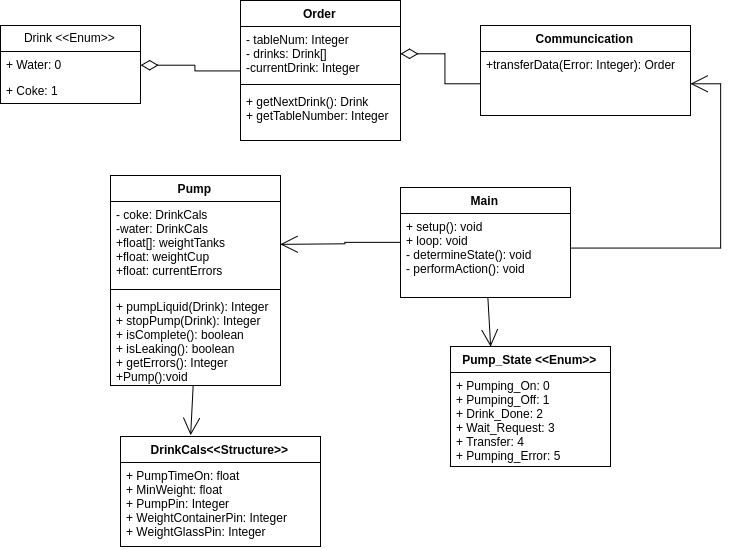
\includegraphics [scale = 0.4] {figures/Pumping_UsesDiagram.png}
	\caption{Uses Relation Diagram for the pumping system}
\end{figure}

% -------------------------------------------------------- MIS ----------------------------------------------------- %

\subsection{MIS}

% ------------------------------- Main Class ---------------------------------- %

\subsubsection{Main Class}

\textbf{Uses}
\begin{itemize}
	\item Order (Class)
	\item Drink (Enum)
	\item Pump (Class)
	\item Pump\_State (Enum)
	\item Communication (Class)
\end{itemize}

\textbf{Internal Variables}
None

\textbf{Functions}

\textbf{public setup(): void}

Setup function for Arduino that initializes the pins that will be used 

\textbf{publicloop(): void}

Main loop that will preform the main logic of the pumping system

\textbf{public determineState(): void}

Based on the previous state of the pumping machine will look at factors such as weight of the liquid, need for communication and errors to determine the next state.

\textbf{public performAction(): void}

Based on the state of the device it will:
\begin{itemize}
	
	\item Pumping\_On: Turn on the voltage for the pump
	\item Pumping\_Off: Turn off the voltage for the pump
	
	\item Wait\_Request: Will Sleep for a specific amount of time before checking again
	\item Transfer: Preform transferring via UART
	\item Pumping\_Error: Perform No Action, and ensure all pumping devices are off
\end{itemize}


% ------------------------------- Class Pump ---------------------------------- %

\subsubsection{Class Pump}

\textbf{Uses}

\begin{itemize}
	\item DrinkCals
\end{itemize}


\textbf{public Functions}

\textbf{Pump():void}

Initializes the values of the pumping module.

\textbf{pumpLiquid(Drink): Integer}

Turns on the pump for the specific drink type. Based on requirement AF1.

\textbf{stopPump(Drink): Integer}

Turns off the pump for the specific drink type. Based on requirement AF5.

\textbf{isComplete(): Boolean}

Determines if the drink has been completely filled or not based. Based on requirement AF5.


\textbf{isLeaking(): Boolean}

Determines if the containers are losing fluid when there is no pumping. Based on requirement NFR22.

\textbf{isSafeTempature()}

Determines if the containers are still storing the liquids are at a safe temperature. Based on requirement AF6.

% ------------------------------- Communication Class ---------------------------------- %

\subsubsection{Communication Class}

\textbf{Uses}

\begin{itemize}
	\item DrinkCals
\end{itemize}

\textbf{Internal Values}
None

\textbf{Functions}

\textbf{transferData(Integer): Order}

Communication performed used  where Orders are received and errors are transferred with the Manager system.

% -------------------------------------------------------- MID ----------------------------------------------------- %

\subsection{MID}

% ------------------------------- Main Class ---------------------------------- %

\subsubsection{Main Class}

\textbf{Uses}
\begin{itemize}
	\item Order (Class)
	\item Drink (Enum)
	\item Pump (Class)
	\item Pump\_State (Enum)
	\item Communication (Class)
\end{itemize}

\textbf{Internal Variables}

 None

\textbf{Functions}

\textbf{public setup(): void}

Setup function for Arduino that initializes the pins that will be used 

\textbf{public loop(): void}

Main loop that will preform the main logic of the pumping system

\textbf{public determineState(): void}

Based on the previous state of the pumping machine will look at factors such as weight of the liquid, need for communication and errors to determine the next state. Which state is summarized in the following table:
\begin{figure} [h!]
	\centering
	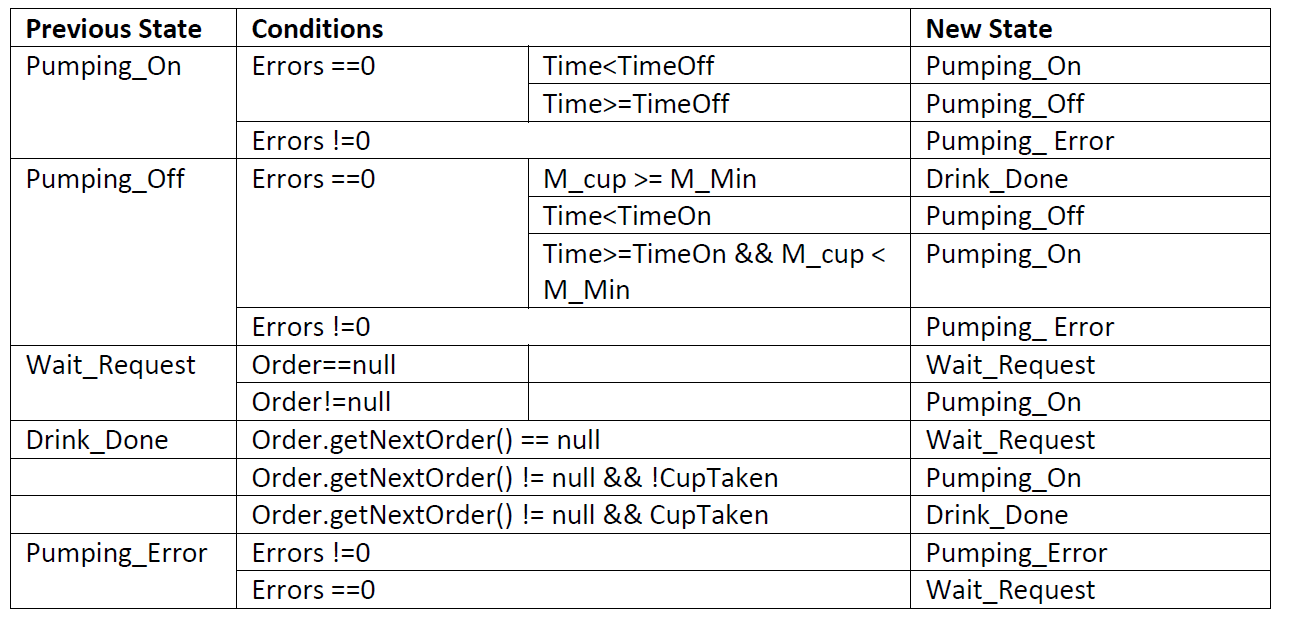
\includegraphics [scale = 0.45] {figures/Pumping_DetermineState.png}
\end{figure}

\textbf{public performAction(): void}

Based on the state of the the pumping system, will preform the following actions:
\begin{figure} [h!]
	\centering
	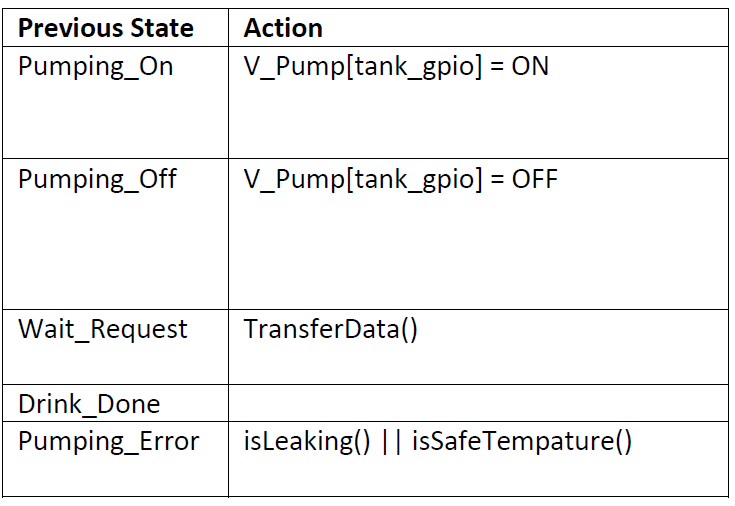
\includegraphics [scale = 0.45] {figures/Pumping_PerformActions.png}
\end{figure}

% ------------------------------- Pump Class ---------------------------------- %

\subsubsection{Pump Class}

\textbf{Uses}

\begin{itemize}
	\item DrinkCals
\end{itemize}

\textbf{Internal Values}

\textbf{DrinkCals coke}: Structure holding the calibrations related to Coke products

\textbf{DrinkCals water}: Structure holding the calibrations related to Water

\textbf{Functions}

\textbf{public Pump():void}

Initializes the values of the pumping module.

\textbf{public pumpLiquid(Drink): Integer}

Turns on the pump for the specific drink type.

\textbf{public stopPump(Drink): Integer}

Turns off the pump for the specific drink type.

\textbf{public isComplete(): Boolean}

Determines if the drink has been completely filled or not based on the following equation:
$Filled := M_min < M_cup$

\textbf{public isLeaking(): Boolean}

Determines if the containers are losing fluid when there is no pumping based on the following equation:
$Leaking := [M_minleak < (M_container1 - M_container_prev1) \wedge Pin7 ==0] \vee [M_minleak < (M_container2 - M_container_prev2) \wedge Pin8 ==0] $

\textbf{public isSafeTempature()}

Determines if the containers are still storing the liquids at a temperature greater then the minimum temperature for the liquids based off of the following equations.
$OverTempature := (T_container1 < T_min) \vee (T_container2 < T_min)$ 

% ------------------------------- Communication Class ---------------------------------- %

\subsubsection{Communication Class}

\textbf{Uses}

\begin{itemize}
	\item DrinkCals
\end{itemize}

\textbf{Internal Values}
 None

\textbf{Functions}

\textbf{transferData(Integer): Order}

Communication performed used using UART where Orders are received and errors are transferred. The first 32 bits will be the errors associated with the pumping system and the last bit will be if the robot is done.



% ------------------------------------------------------- SERVER ----------------------------------------------------- %

\section {Server}

% ---------------------------------------------- Purpose --------------------------------------------- %

\subsection{Purpose}
The following will describe the component software design associated with the server. This system will be run on an external RHEL server.

% ---------------------------------------------- Scope --------------------------------------------- %

\subsection{Scope}
The scope of this section is associated with the REST API server that will be responsible for the communication within the system. The software documentation will provide the MIS and MID, uses relations to describe how the system will be designed to perform its function of being able to route communication between difference modules in the system.

% ---------------------------------- Module Decomposition --------------------------------- %

\subsection{Module Decomposition}
\textbf{Serer Module}: Will have different REST API endpoints available to be able to "perform actions" in different parts of the system, as well as route data.

% ----------------------------------- Uses Relation ------------------------------------- %

\pagebreak

\subsection{Uses Relation}
\begin{figure} [h!]
	\centering
	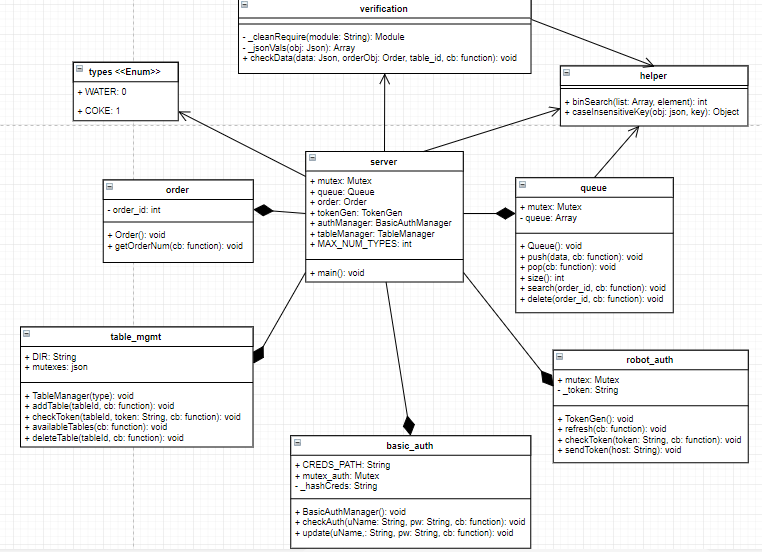
\includegraphics [scale = 0.55] {figures/server_class_diagram.PNG}
	\caption{Alfred Uses Relation Diagram}
\end{figure}

% -------------------------------------------------------- MIS ----------------------------------------------------- %

\subsection{MIS}

% ------------------------------- Server ---------------------------------- %

\subsubsection{server}
\textbf{Uses}
\begin{itemize}
	\item order (Class)
	\item types (Enum)
	\item verification (Class)
	\item helper (Class)
	\item queue (Class)
	\item robot\_auth (Class)
	\item basic\_auth (Class)
	\item table\_mgmt (Class)
	\item http (External Class)
	\item url (External Class)
	\item fs (External Class)
	\item locks (External Class)
\end{itemize}

\textbf{Public Functions}
\textbf{main(): void}
Running the server, intercepting REST API requests and taking required action.

% ------------------------------- Queue ---------------------------------- %

\subsubsection{queue}
\textbf{Uses}
\begin{itemize}
	\item locks (External Class)
	\item helper (Class)
\end{itemize}

\textbf{Public Functions}
\textbf{Queue(): void}
Constructor function that creates a new empty queue.

\textbf{push(data, cb): void}
Push new order information into the queue and callback function with the place in line.

\textbf{pop(cb): void}
Pops the first element from the queue.

\textbf{size(): int}
calls the callback function with the current size of the queue.

\textbf{search(order\_id, cb): void}
Searches the queue and calls callback function with the place in line for the order specified by the order\_id.

\textbf{delete(order\_id, cb): void}
Searches the queue for order identified by given order\_id and removes it from the queue.

% ------------------------------- helper ---------------------------------- %

\subsubsection{helper}
\textbf{Uses}
None

\textbf{Public Functions}
\textbf{binSearch(list, element): int}
Binary search algorithm to find an element and return its position. If element not found, returns -1.

\textbf{caseInsensitiveKey(obj, key): obj[i]}
Extracts information from a JSON object for a given key. Comparison between the key and the JSON object's keys are case insensitive.

% ------------------------------- basic/ auth ---------------------------------- %

\subsubsection{basic\_auth}
\textbf{Uses}
\begin{itemize}
	\item fs (External Class)
	\item locks (External Class)
	\item util (External Class)
	\item crypto (External Class)
\end{itemize}

\textbf{Public Functions}
\textbf{BasicAuthManager(): void}
Constructor function to create the object.

\textbf{checkAuth(uName, pw, cb): void}
Will check the validity of the username and password given as parameters, and will call the callback function with a boolean of whether username/password combination is valid.

\textbf{update(uName, pw, cb): void}
Will update the stored username and password combination, with the given ones.

% ------------------------------- robot/ auth ---------------------------------- %

\subsubsection{robot\_auth}
\textbf{Uses}
\begin{itemize}
	\item locks (External Class)
	\item rand-token (External Class)
	\item unirest (External Class)
\end{itemize}

\textbf{Public Functions}
\textbf{TokenGen(): void}
Constructor function to create the object with new token.

\textbf{refresh(cb): void}
Updates current token.

\textbf{checkToken(token, cb): void}
Check that the given token in the parameters matches the token stored in the object, and calls the callback function with boolean result.

\textbf{sendToken(host): void}
Will send current token to the 'host' given in the parameters.

% ------------------------------- verification ---------------------------------- %

\subsubsection{verification}
\textbf{Uses}
\begin{itemize}
	\item helper (Class)
	\item types (Enum)
\end{itemize}

\textbf{Public Functions}
\textbf{checkData(data, orderObj, table\_id, cb): void}
Verify that the order information in the HTTP request has all necessary information and is in the correct format. Information required includes drink types, sizes, and quantities. Then calls callback function with error, if one exists.

% ------------------------------- table management ---------------------------------- %

\subsubsection{table\_mgmt}
\textbf{Uses}
\begin{itemize}
	\item locks (External Class)
	\item rand-token (External Class)
	\item fs (External Class)
	\item crypto (External Class)
\end{itemize}

\textbf{Public Functions}
\textbf{TableManager(): void}
Constructor function that reads all currently listed tables from the tables filesystem and creates a mutex for each.

\textbf{addTable(tableId, cb): void}
Register a new table with the filesystem and generate an authentication token for that table to be used with server communication, then calls the callback function with the token.

\textbf{checkToken(tableId, token, cb): void}
Verify that an inputted token is correct for the table, and calls callback function with boolean result.

\textbf{availableTables(cb): void}
Search the filesystem to find all tables currently registered, and call callback function with list of all tables.

\textbf{deleteTable(tableId, cb): void}
Remove a table from the filesystem.

% ------------------------------- order ---------------------------------- %

\subsubsection{order}
\textbf{Uses}
\begin{itemize}
	\item locks (External Class)
\end{itemize}

\textbf{Public Functions}
\textbf{Order(): void}
Constructor function that creates a new Order object, with order\_id == 0.

\textbf{getOrderNum(cb): void}
Call the callback function with the next order\_id and increment the counter.

% -------------------------------------------------------- MID ----------------------------------------------------- %

\subsection{MID}

% ------------------------------- server ---------------------------------- %

\subsubsection{server}
\textbf{Uses}
\begin{itemize}
	\item order (Class)
	\item types (Enum)
	\item verification (Class)
	\item helper (Class)
	\item queue (Class)
	\item robot\_auth (Class)
	\item basic\_auth (Class)
	\item table\_mgmt (Class)
	\item http (External Class)
	\item url (External Class)
	\item fs (External Class)
	\item locks (External Class)
\end{itemize}

\textbf{Internal Values}
\begin{itemize}
	\item Mutex mutex: Mutex to synchronize requests updating value of 'types.json' in the filesystem.
	\item Queue queue: A FIFO queue where orders are stored.
	\item Order order: Object to keep track of order ID's.
	\item TokenGen tokenGen: A token generator and manager for the robot token for authentication.
	\item BasicAuthManager authManager: Object responsible for authenticating administrator.
	\item TableManager tableManager: Object responsible for authenticating each table.
	\item final int MAX\_NUM\_TYPES: Variable storing maximum number of types of drinks that the robot can hold.
\end{itemize}

\textbf{Functions}
\textbf{main(): void}

\begin{center}
	\begin{tabular}{ |c|c|c| } 
		\hline
		\textbf{GET} & \textbf{POST} & \textbf{DELETE} \\ \hline
		placeinline & placeorder & cancelorder \\ \hline
		nextorder & gentoken & drinks \\ \hline
		checktoken & updatecreds & tables \\ \hline
		drinks & returntobase &  \\ \hline
		sizes & login &  \\ \hline
		numoftanks & errors &  \\ \hline
		& drinks &  \\ \hline
		& tables &  \\ \hline
	\end{tabular}
\end{center}

\textbf{Placeinline}
Call checkToken for table authentication
If passed, search queue for order\_id
res.write(placeInLine.toString());
\newline\textbf{Placeorder}
Call checkToken for table authentication
If passed, parse the body of the request
Verify that all data is correct
If correct, push order to queue
\newline\textbf{cancelOrder}
Call checkToken for robot authentication
If passed, delete order from queue for specific order\_id
\newline\textbf{Nextorder}
Call checkToken for robot authentication
If passed, call queue's pop function
res.write(placeInLine.toString());
\newline\textbf{Gentoken}
Call token refresh function
Send token to robot host
\newline\textbf{Checktoken}
Call checkToken for robot authentication
res.write(JSON.stringify(resp\_auth));
\newline\textbf{Updatecreds}
Call checkAuth for admin authentication
If passed, parse body of request
Call authManager update function to update new user/password combination
\newline\textbf{Login}
Call checkAuth for admin authentication
res.writeHead(200, 'Logged in', {'Content-Type': 'text/html'}); if credentials were authenticated
\newline\textbf{Returntobase}
Call checkAuth for admin authentication
Call returnToBase function to have robot return to the kitchen
\newline\textbf{Sizes}
Print out list of drinks that are available
\newline\textbf{Numoftanks}
Print out maximum number of tanks that the robot can hold
\newline\textbf{Errors}
Call checkToken for robot authentication
If passed, list all error messages thrown by the robot
\newline\textbf{Drinks (GET)}
Print out list of drinks that are available
\newline\textbf{Drinks (POST)}
Call checkAuth for admin authentication
Check that the total number of drink types is not already at the maximum
Parse the body of the request
Lock mutex
Store new drink type and tank number into drinks object and write them to file
Unlock mutex
\newline\textbf{Drinks (DELETE)}
Call checkAuth for admin authentication
If passed, parse body of the request. Lock the mutex
Delete specified drink type from DRINKS object. Write drink type list to file
Unlock the mutex
\newline\textbf{Tables (POST)}
Call checkAuth for admin authentication
If passed, call addTable function
res.write(JSON.stringify({token: token, token\_type: 'bearer'}));
\newline\textbf{Tables (DELETE)}
Call checkAuth for admin authentication
If passed, call deleteTable function

% ------------------------------- queue ---------------------------------- %

\subsubsection{queue}
\textbf{Uses}
\begin{itemize}
	\item locks (External Class)
	\item helper (Class)
\end{itemize}

\textbf{Internal Values}
\begin{itemize}
	\item Mutex mutex: Mutex used to lock the resource to prevent from problems arising from asynchronicity.
	\item Array queue: An array to store elements in queue.
\end{itemize}

\textbf{Functions}
\textbf{Queue(): void}
This.queue = []

\textbf{push(data, cb): void}
Lock queue
Add data to the queue
Unlock queue
cb(null, length of queue)

\textbf{pop(cb): void}
Lock queue
element = queue.pop()
Unlock queue
cb(null, element)

\textbf{size(): int}
Return queue.length

\textbf{search(order\_id, cb): void}
index = helper.binSearch(queue, order\_id)
if (index >= 0) {
	cb(null, (that.queue.length - index));
} else {
	cb('order\_id not in queue');
}

\textbf{delete(order\_id, cb): void}
Lock queue
index = helper.binSearch(queue, order\_id)
Remove element from queue at index if it exists
cb()

% ------------------------------- helper ---------------------------------- %

\subsubsection{helper}
\textbf{Uses}
None

\textbf{Internal Values}
None

\textbf{Functions}
\textbf{binSearch(list, element): int}
Binary search algorithm based on element being the order\_id.
Return index if found or -1 if not found

\textbf{caseInsensitiveKey(obj, key): obj[i]}
For k in keys of obj
	If k.toLowerCase() == key.toLowerCase()
		Return obj[k]
Return null

% ------------------------------- basic auth ---------------------------------- %

\subsubsection{basic\_auth}
\textbf{Uses}
\begin{itemize}
	\item fs (External Class)
	\item locks (External Class)
	\item util (External Class)
	\item crypto (External Class)
\end{itemize}

\textbf{Internal Values}
\begin{itemize}
	\item Mutex mutex\_auth: Mutex to synchronize token from asynchronicity.
	\item final String CREDS\_PATH: Path to store hashed credentials in.
	\item String \_hashCreds: Hashed value of current user credentials.
\end{itemize}

\textbf{Functions}
\textbf{BasicAuthManager(): void}
If CREDS\_PATH exists
	\_hashCreds = readFile(CREDS\_PATH)
Else
	\_hashCreds = hash('admin:admin')
	writeToFile(CREDS\_PATH, \_hashCreds)

\textbf{checkAuth(uName, pw, cb): void}
mutex\_auth.lock()
passed = \_hashCreds == hash(uName + ':' + pw)
mutex\_auth.unlock()
cb(null, passed)

\textbf{update(uName, pw, cb): void}
mutex\_auth.lock()
\_hashedCreds =  hash(uName + ':' + pw)
writeToFile(CREDS\_PATH, \_hashedCreds)
mutex\_auth.unlock()
cb()

% ------------------------------- robot auth ---------------------------------- %

\subsubsection{robot\_auth}
\textbf{Uses}
\begin{itemize}
	\item locks (External Class)
	\item rand-token (External Class)
	\item unirest (External Class)
\end{itemize}

\textbf{Internal Values}
\begin{itemize}
	\item Mutex mutex: Mutex to synchronize token from asynchronicity.
	\item String \_token: Value of current token to authenticate robot.
\end{itemize}

\textbf{Functions}
\textbf{TokenGen(): void}
\_token = rand-token.generate(32)

\textbf{refresh(cb): void}
mutex.lock()
\_token = rand-token.generate(32)
mutex.unlock()
cb()

\textbf{checkToken(token, cb): void}
mutex.lock()
passed = token == \_token
mutex.unlock()
cb(null, passed)

\textbf{sendToken(host): void}
data = {
	token\_type: 'bearer',
	access\_token : \_token
}
unirest.post(host, data)

% ------------------------------- verification ---------------------------------- %

\subsubsection{verification}
\textbf{Uses}
\begin{itemize}
	\item helper (Class)
	\item types (Enum)
\end{itemize}

\textbf{Internal Values}
None

\textbf{Functions}
\textbf{checkData(data, orderObj, table\_id, cb): void} \newline
order = helper.caseInsensitiveKey(data, 'order') \newline
If order missing values or in wrong format  \newline
	cb(error) \newline
\newline
orders = [] \newline
\newline
For i of order \newline
	temp = {} \newline
	type = helper.caseInsensitiveKey(i, 'type') \newline
	size = helper.caseInsensitiveKey(i, 'size') \newline
	quantity =  helper.caseInsensitiveKey(i, 'quantity') \newline
	If type is valid \newline
		temp.type = type \newline
	Else \newline
		Continue \newline
	 \newline
	If size valid \newline
		temp.size = size \newline
	Else \newline
		Temp.size = M \newline
	If quantity valid \newline
		temp.quantity  = quantity \newline
	Else \newline
		temp.quantity  = 1 \newline
	\newline
	orders.push(temp) \newline
\newline
If no orders \newline
	Return cb(no valid 'orders') \newline
\newline
orderObj.getOrderNum(function(err, order\_id) { \newline
	if (err) { \newline
		return cb(err); \newline
	} \newline
	//return order information \newline
	cb(null, { \newline
		table\_id: table\_id, \newline
		order\_id: order\_id, \newline
		orders: orders \newline
	}); \newline
}); \newline
 \newline
\textbf{\_cleanRequire(module): Module} \newline
Delete cached data for module \newline
Return require(module) \newline
 \newline
\textbf{\_jsonVals(obj): Array} \newline
ret = [] \newline
For i of Object.keys(obj) \newline
	ret.push(obj[i]) \newline
Return ret \newline

\subsubsection{table\_mgmt}
\textbf{Uses}
\begin{itemize}
	\item locks (External Class)
	\item rand-token (External Class)
	\item fs (External Class)
	\item crypto (External Class)
\end{itemize}

\textbf{Internal Values}
\begin{itemize}
	\item final String DIR: Directory to store hashed tokens for tables
	\item Json mutexes: A mutex for each table, to synchronize tokens from asynchronous calls.
\end{itemize}

\textbf{Functions}
\textbf{TableManager(): void}
Create DIR filesystem if not already created
Read all files from filesystem, create a mutex for each, and load the filename/mutex pairs into a JSON object

\textbf{addTable(tableId, cb): void}
Create new mutex for new table and add to JSON object
Lock mutex for new table
Create new file in tables filesystem
Generate authentication token for table
Write hashed token to corresponding file in tables filesystem
Unlock mutex for table
cb(null, token)

\textbf{checkToken(tableId, token, cb): void}
Verify that an inputted token is correct for the table, and calls callback function with boolean result.

\textbf{availableTables(cb): void}
Read all files from filesystem
cb(null, files)

\textbf{deleteTable(tableId, cb): void}
Lock mutexes JSON object
Unlink table's path from filesystem
Delete mutexes[tableId]
Unlock JSON object
cb()

% ------------------------------- order ---------------------------------- %

\subsubsection{order}
\textbf{Uses}
\begin{itemize}
	\item locks (External Class)
\end{itemize}

\textbf{Internal Values}
\begin{itemize}
	\item int order\_id: Current order number.
\end{itemize}

\textbf{Public Functions}
\textbf{Order(): void}
This.order\_id = 0

\textbf{getOrderNum(cb): void}
Lock counter
Add one to counter
Unlock counter
cb(null, new order\_id)


% ------------------------------------------------------- SCHEDULING ----------------------------------------------------- %


\section {Scheduling}

\begin{figure}[h!]
	\centering
	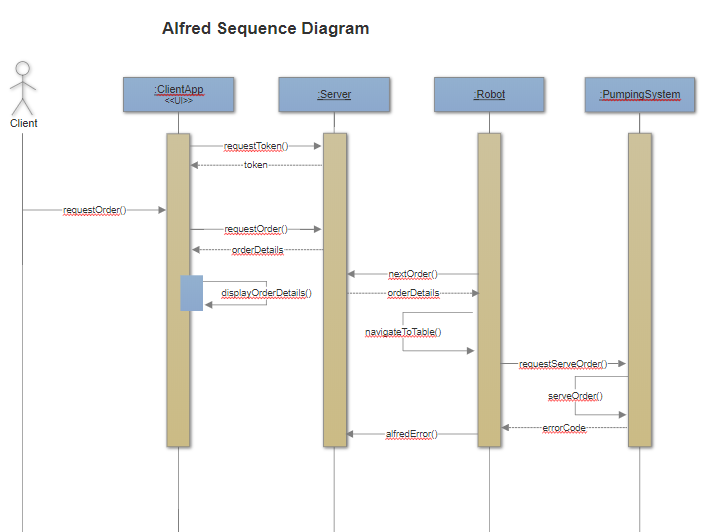
\includegraphics [scale = 0.6] {figures/Alfred_SequenceDiagram.png}
	\caption{Alfred Sequence Diagram}
\end{figure}

\newpage

% ------------------------------------------------------- DESIGN NOTES ----------------------------------------------------- %

\section {Design Notes}

\begin{figure}[H]
	\centering
	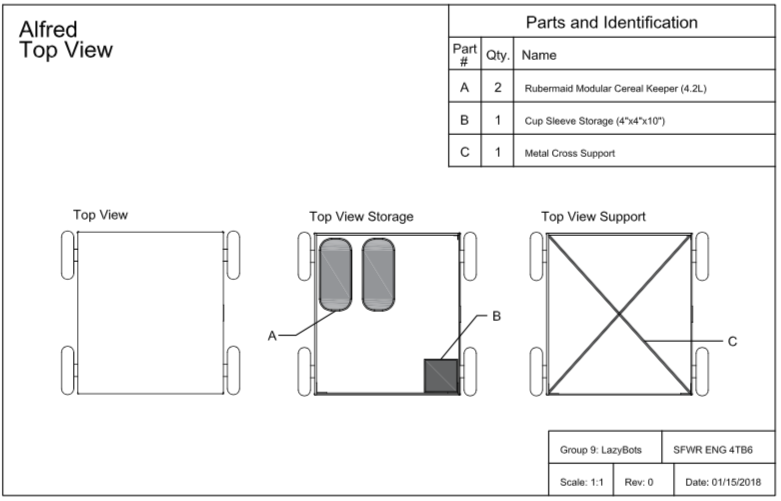
\includegraphics [scale = 0.55] {figures/CAD_Top_View.png}
	\caption{Engineering Model - Top View}
\end{figure}
	
\begin{figure}[H]
	\centering
	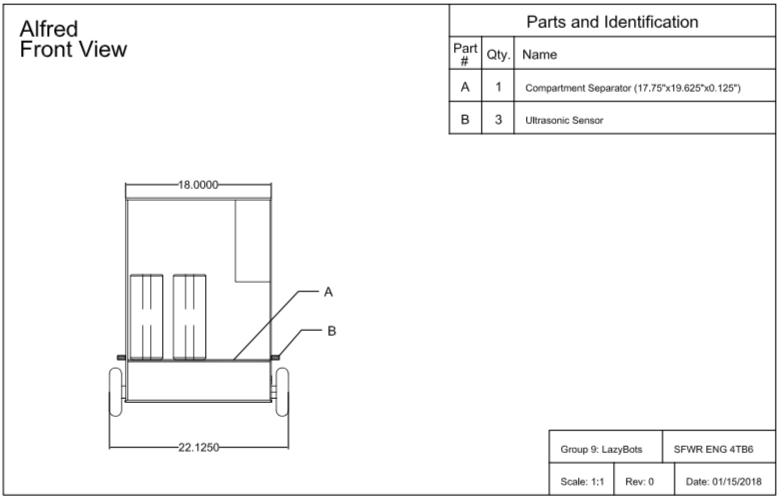
\includegraphics [scale = 0.55] {figures/CAD_Front_View.png}
	\caption{Engineering Model - Front View}
\end{figure}
	
\begin{figure}[H]
	\centering
	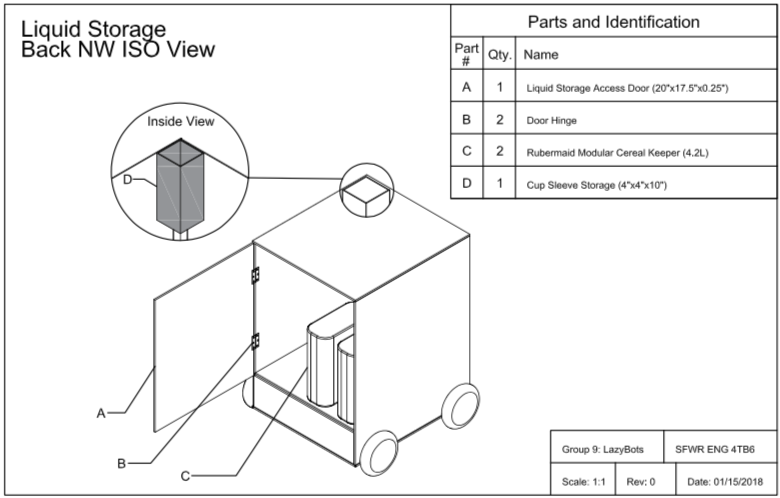
\includegraphics [scale = 0.55] {figures/CAD_Liquid_Storage.png}
	\caption{Engineering Model - Liquid Storage}
\end{figure}

\begin{figure}[H]
	\centering
	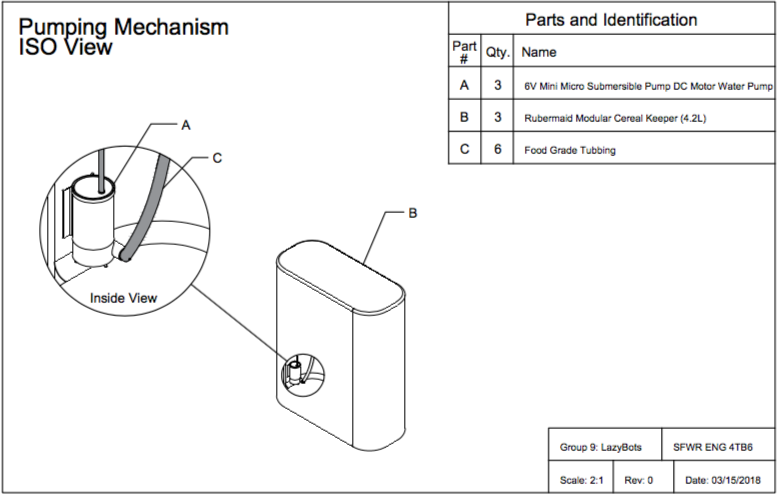
\includegraphics [scale = 0.55] {figures/CAD_Pumping_System.png}
	\caption{Engineering Model - Pumping System}
\end{figure}
	
\begin{figure}[H]
	\centering
	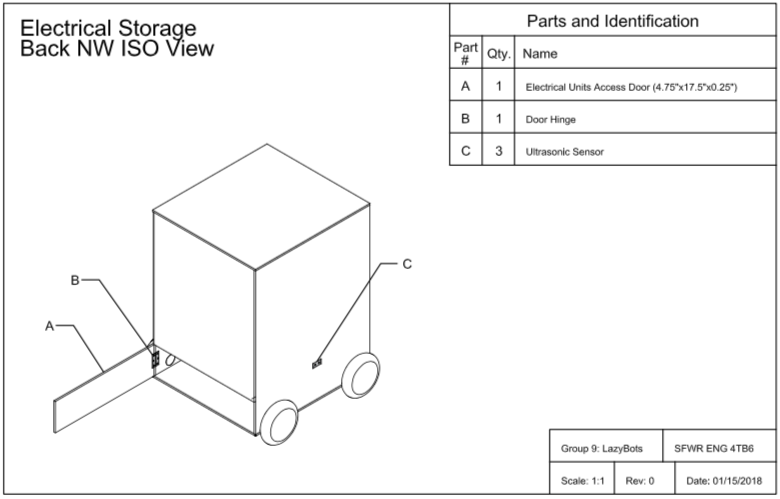
\includegraphics [scale = 0.55] {figures/CAD_Electrical_Storage.png}
	\caption{Engineering Model - Electrical Storage}
\end{figure}
	
\begin{figure}[H]
	\centering
	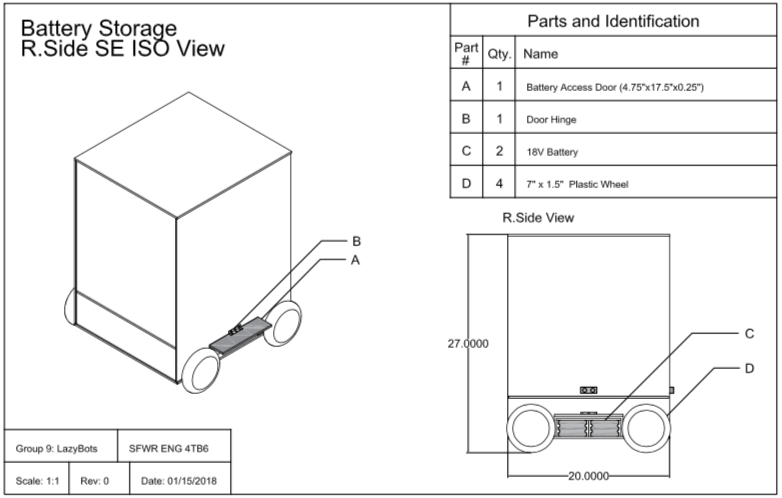
\includegraphics [scale = 0.55] {figures/CAD_Battery_Storage.png}
	\caption{Engineering Model - Battery Storage}
\end{figure}
	
\begin{figure}[H]
	\centering
	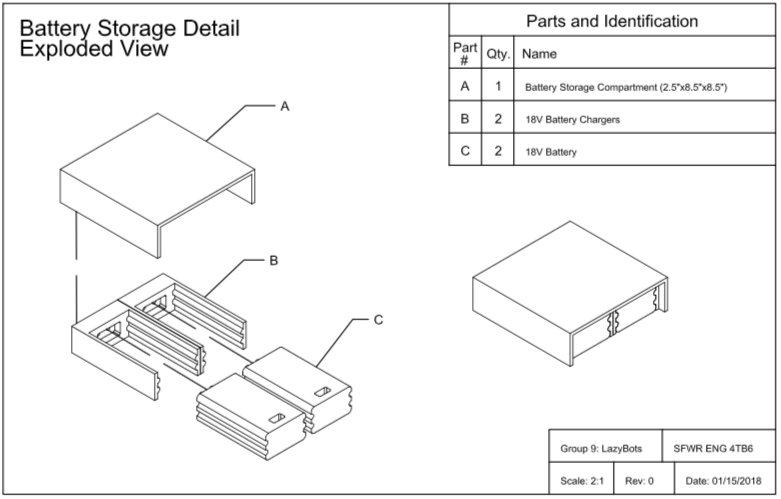
\includegraphics [scale = 0.55] {figures/CAD_Battery.png}
	\caption{Engineering Model - Battery Compartment Exploded View}
\end{figure}

\begin{figure}[H]
	\centering
	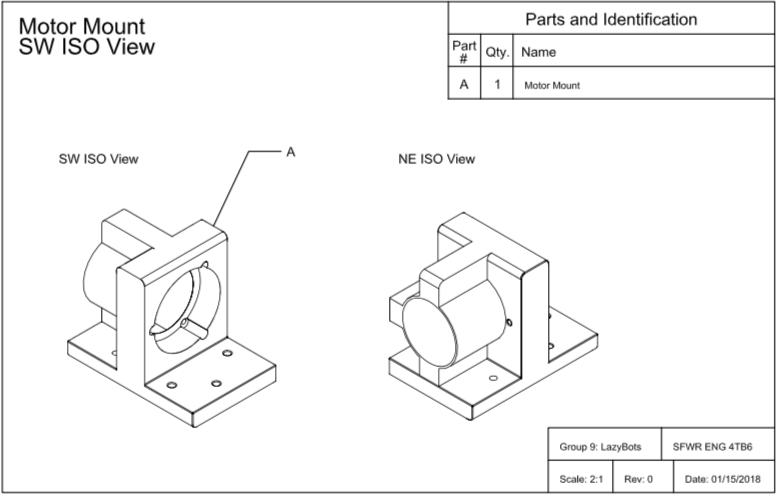
\includegraphics [scale = 0.55] {figures/CAD_Motor_Mount.png}
	\caption{Engineering Model - Motor Mount}
\end{figure}

\begin{figure}[H]
	\centering
	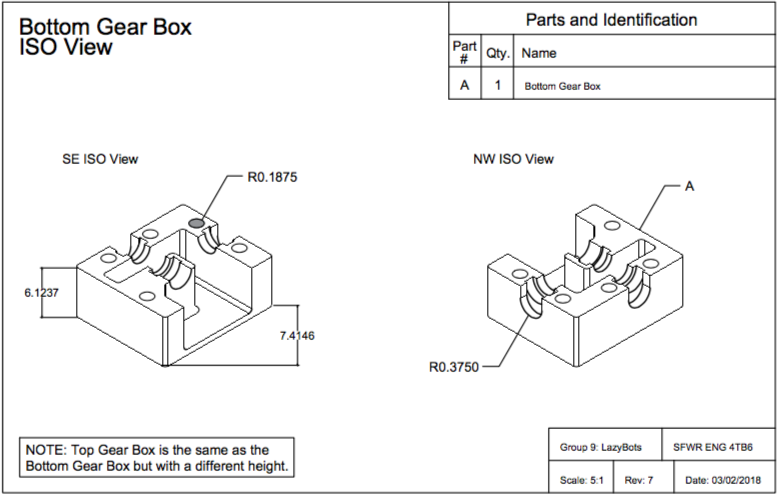
\includegraphics [scale = 0.55] {figures/CAD_Bottom_GB.png}
	\caption{Engineering Model - Bottom Gear Box}
\end{figure}

\begin{figure}[H]
	\centering
	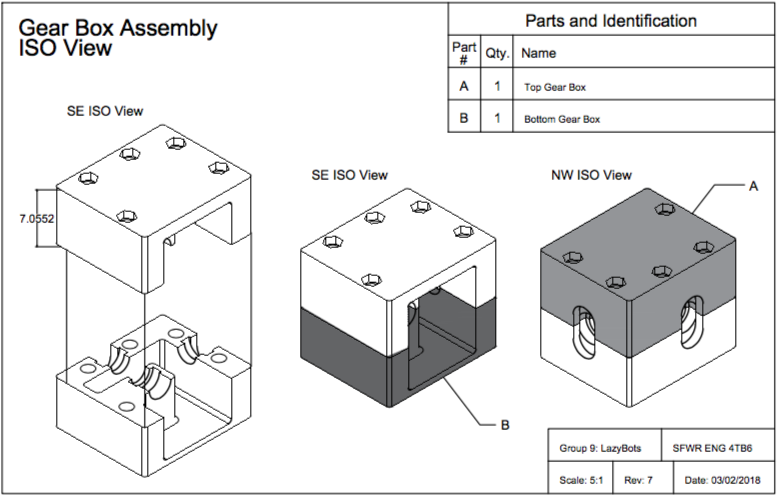
\includegraphics [scale = 0.55] {figures/CAD_GB_Assembly.png}
	\caption{Engineering Model - Gear Box Assembly}
\end{figure}

\begin{figure}[H]
	\centering
	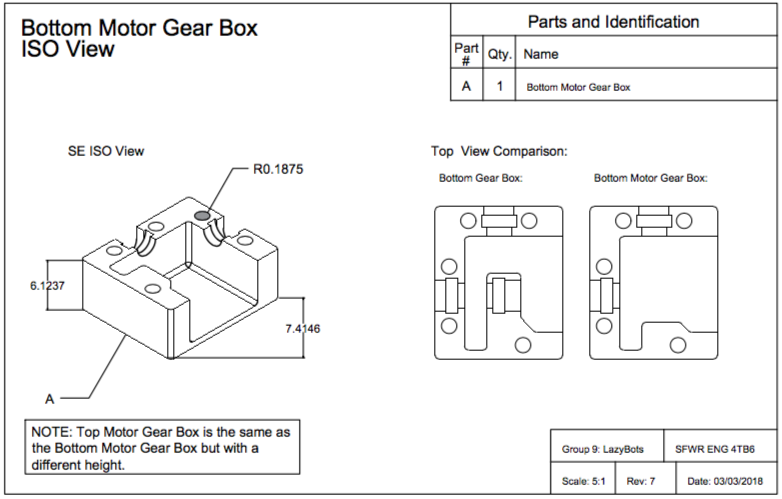
\includegraphics [scale = 0.55] {figures/CAD_Bottom_Motor_GB.png}
	\caption{Engineering Model - Gear Box Assembly}
\end{figure}

\begin{figure}[H]
	\centering
	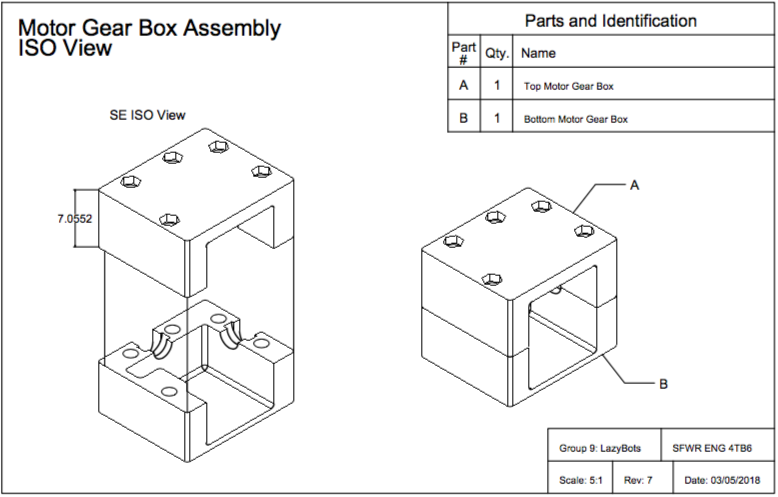
\includegraphics [scale = 0.55] {figures/CAD_Motor_GB.png}
	\caption{Engineering Model - Bottom Motor Gear Box}
\end{figure}


% --------------------------------------------- References -------------------------------------------- %

\pagebreak

\section{References}

\textbf{Raspberry pi data sheet}
\begin{verbatim}
[1]"Exploring Raspberry Pi", 2017. [Online]. 
Available: http://docs-europe.electrocomponents.com/webdocs/14ba/0900766b814ba5fd.pdf. 
[Accessed: 23- Dec- 2017].
\end{verbatim}

\textbf{Arduino Mega Information}
\begin{verbatim}
[2] "Arduino Mega". [Online]. Available:
https://www.arduino.cc/en/Main/ArduinoBoardMega. [Accessed: 23- Dec- 2017].
\end{verbatim}

\textbf{DC Pump Information}
\begin{verbatim}
[3] "3-6V Mini Micro Submersible Pumps DC Motor Pump Water Pump - 80-120L/H". [Online]. 
Available: 
https://www.amazon.ca/gp/product/B01LWQCXEL/ref=oh_aui_detailpage_o02_s00?ie=UTF8&psc=1.
[Accessed: 23- Dec- 2017].
\end{verbatim}
\textbf{Pump Container Information}
\begin{verbatim}
[4] "Rubbermaid 1856059 Modular Cereal Keeper". [Online]. 
Available: 
https://www.amazon.ca/gp/product/B00BEUDXRW/ref=oh_aui_detailpage_o09_s00?ie=UTF8&psc=1. 
[Accessed: 23- Dec- 2017].
\end{verbatim}

\textbf{Raspberry camera pi data sheet}
\begin{verbatim}
[4] "CAMERA MODULE". [Online]. Available:
https://www.raspberrypi.org/documentation/hardware/camera/. [Accessed: 23- Dec- 2017].
\end{verbatim}


\end{document}
